% TODO
% Deben incluir los resultados de los experimentos, utilizando el formato mas adecuado
% para  su  presentacion.   Deberan  especicar  claramente  a  que  experiencia  corresponde
% cada resultado.  No se incluiran aqu corridas de maquina.
\subsection{Performance}
\subsubsection{Gauss vs LU para una sola instancia variando discretizaciones}

Se generaron diversas discretizaciones, fijando la cantidad de \'angulos en 30, y variando la cantidad de radios de 5 a 30, con una instancia para cada discretizaci\'on. El objetivo es analizar la evoluci\'on del tiempo de c\'omputo a mayor granulaidad de la discretizaci\'on, y comprobar emp\'iricamente que la complejidad de ambos algoritmos es del orden c\'ubico.

  	\textbf{Perfomance de factorizai\'on LU para distinta granularidad de radios}\\

\begin{center}
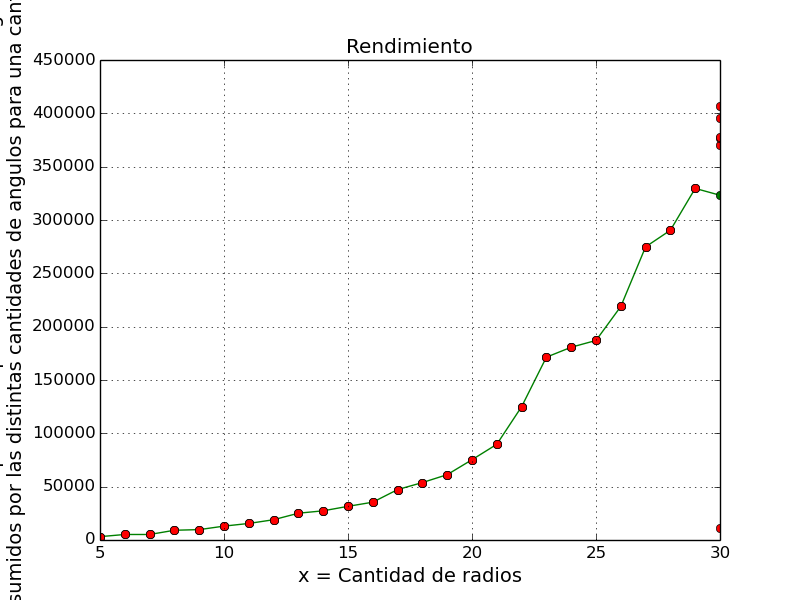
\includegraphics[scale=0.65]{experimentos2a_2b/gaussMed.png}
\end{center}

  	\textbf{Perfomance de Gauss para distinta granularidad de radios}\\

\begin{center}
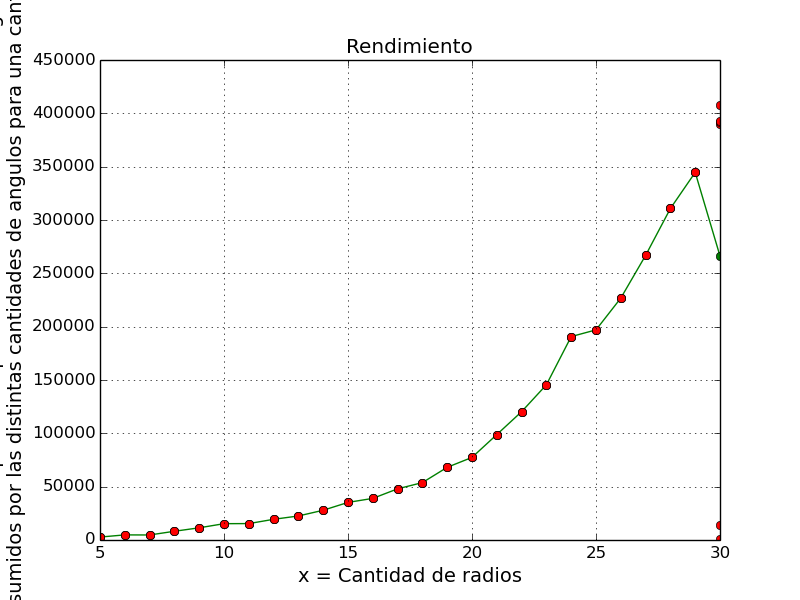
\includegraphics[scale=0.65]{experimentos2a_2b/Lumed.png}
\end{center}

A continuaci\'on, usaremos una heur\'istica para poder determinar mejor el orden c\'ubico de la curva resultado. Esta es, sea $x$ el valor del tiempo de c\'omputo, dividir $x/f(x)$, siendo $f(x)$ polinomio de orden $2$ y $3$. De ser de orden c\'ubica la curva, esperar\'iamos que para el polinomio de orden 2 el resultado se asemeje a una funci\'on lineal, y para el de orden 3 el resultado se asemeje a una constante.

  	\textbf{Perfomance de factorizai\'on LU sobre cuadrado}\\

\begin{center}
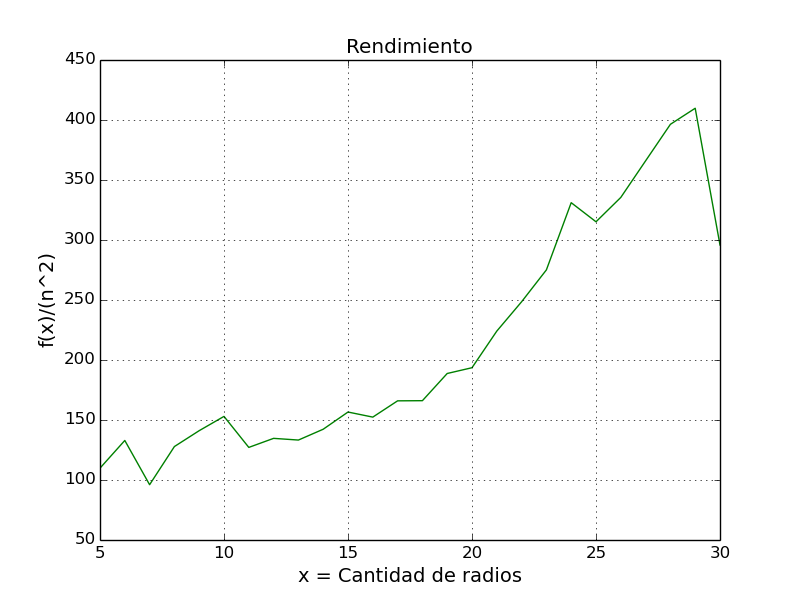
\includegraphics[scale=0.65]{experimentos2a_2b/Lucuadrado.png}
\end{center}

  	\textbf{Perfomance de Gauss sobre cuadrado}\\

\begin{center}
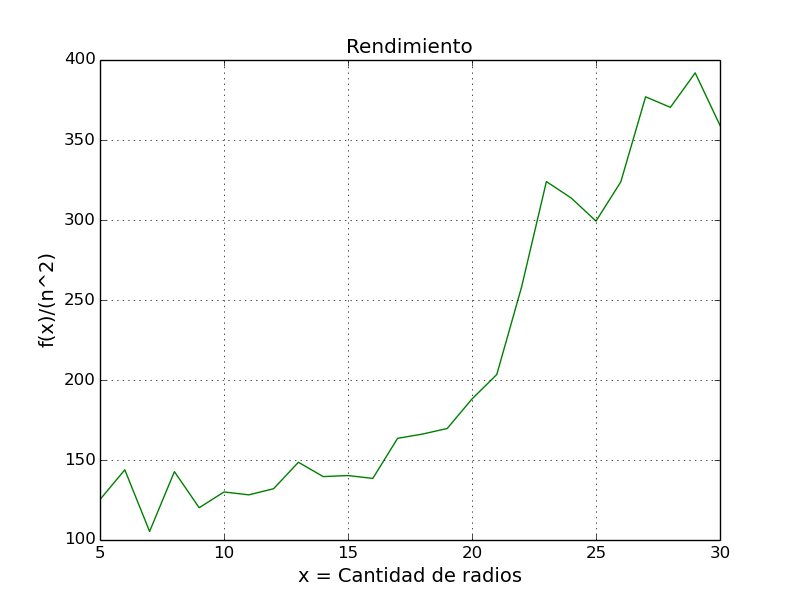
\includegraphics[scale=0.65]{experimentos2a_2b/GaussCuadrado.png}
\end{center}

 \textbf{Perfomance de factorizai\'on LU sobre cubo}\\


\begin{center}
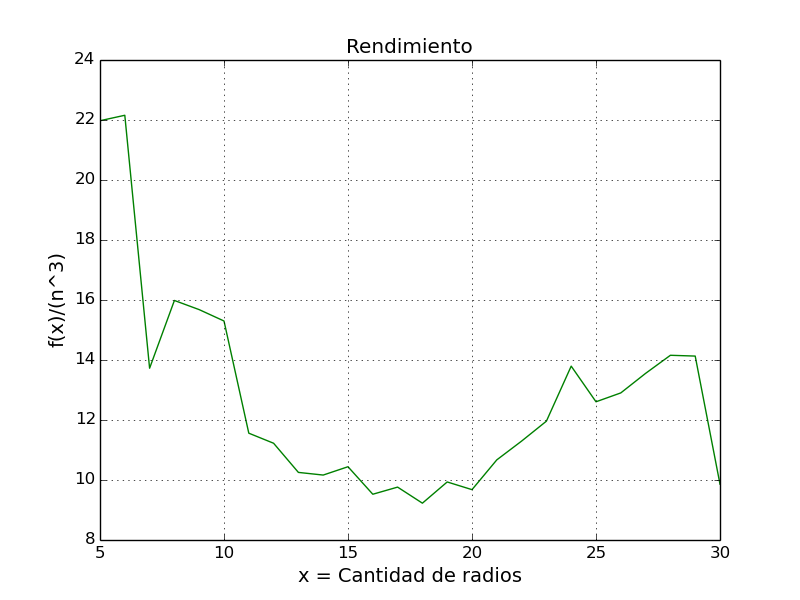
\includegraphics[scale=0.65]{experimentos2a_2b/LuCubo.png}
\end{center}

 \textbf{Perfomance de Gauss sobre cubo}\\


\begin{center}
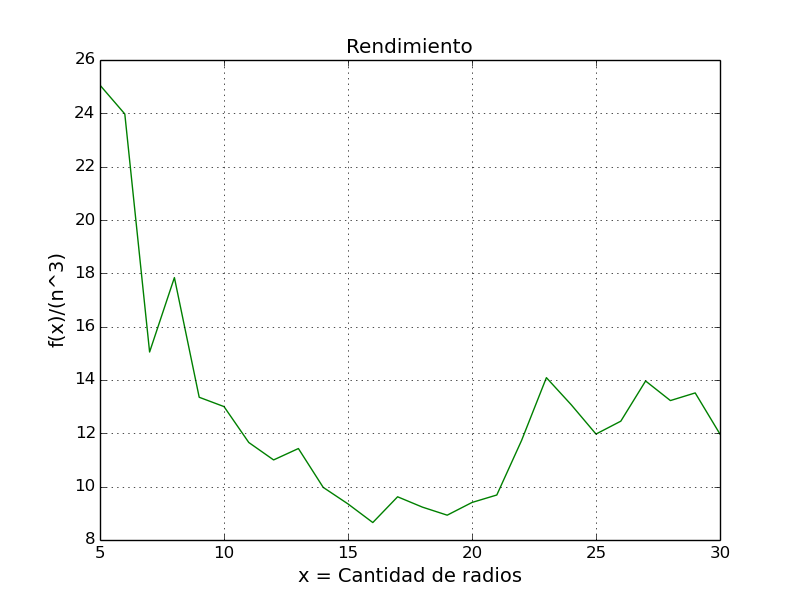
\includegraphics[scale=0.65]{experimentos2a_2b/GaussCubo.png}
\end{center}



\subsubsection{Gauss vs LU para varias instancias de una misma discretizacion}

Para una misma discretizaci\'on elegida de 30 \'angulos y 30 radios, se generaron 3 archivos con distinto n\'umero de instancias, el primero de una instancia, el segundo de 5 instancias, y el tercero de 10. En cada instancia cambian las condiciones de borde. Se medir\'a el tiempo total de ejecuci\'on de cada uno de los dos m\'etodos para cada archivo, de forma de poder comparar la perfomance de ambos m\'etodos bajo una misma discretizaci\'on, variando la cantidad de instancias a resolver.

\vspace{0.5cm}

  	\textbf{Comparaci\'on de Perfomance para una instancia}\\
\begin{center}
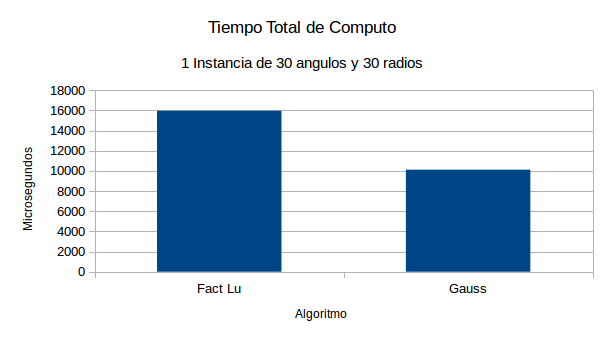
\includegraphics[scale=0.7]{experimentos2a_2b/2bUnaInstancia.png}
\end{center}

Puede verse claramente como, comparando por una instancia, la mayor constante en la complejidad te\'orica de la factorizaci\'on LU se refleja en la experimentaci\'on. \textbf{Ratio LU/Gauss: 1.577}

 \textbf{Comparaci\'on de Perfomance para cinco instancias}\\
\begin{center}
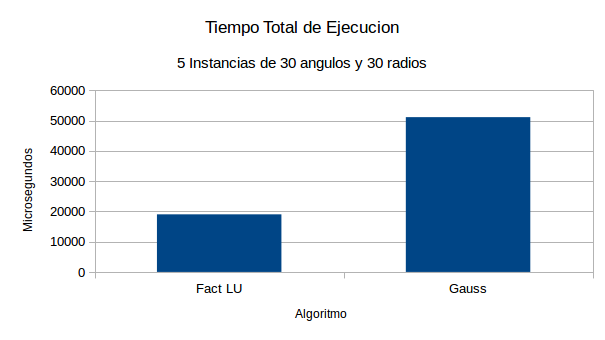
\includegraphics[scale=0.7]{experimentos2a_2b/2bCincoInstancias.png}
\end{center}

Con aumentar en nada m\'as que 4 el n\'umero de instancias, ya se nota una amplia mejora en el tiempo de c\'omputo de factorizaci\'on LU, ya que, al no variar la discretizaci\'on y variar las temperaturas externas e internas, se hace uso al m\'aximo de la mayor ventaja del algoritmo de factorizac\'on LU: para una misma matriz A (discretizaci\'on), y distintas temperaturas (cambia el vector V), luego de la primera vez que resuelve el sistema (que cuesta $O(n^3)$), las subsiguientes veces cuesta $O(n^2)$, dado que simplemente tiene que realizar substituciones. \textbf{Ratio LU/Gauss: 0.3178}

 \textbf{Comparaci\'on de Perfomance para diez instancias}\\
\begin{center}
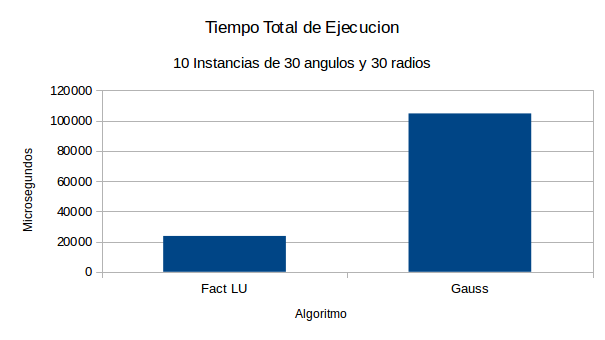
\includegraphics[scale=0.7]{experimentos2a_2b/2bDiezInstancias.png}
\end{center}

Al aumentar el n\'umero de instancias se sigue notando la misma tendencia, y el ratio de mejora de LU sobre Gauss se hace m\'as pequeño a medida que crece el n\'umero de instancias. \textbf{Ratio LU/Gauss: 0.2264}

\subsubsection{Gauss vs LU para 50 instancias variando discretizaciones}

Se compara la perfomance de ambos m\'etodos en el caso opuesto al anterior. Dado un n\'umero fijo de 50 instancias, se medir\'a el tiempo total de c\'omputo en tres discretizaciones: 20 \'angulos y 20 radios, 40 \'angulos y radios, y 60 \'angulos y radios. 

  	\textbf{Comparaci\'on de Perfomance para 20 \'angulos y radios }\\
\begin{center}
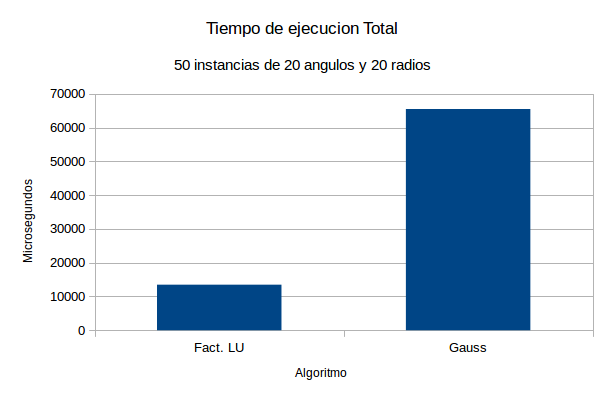
\includegraphics[scale=0.7]{experimentos2a_2b/2b2020.png}
\end{center}

 \textbf{Ratio LU/Gauss: 0.2059}

  	\textbf{Comparaci\'on de Perfomance para 40 \'angulos y radios }\\
\begin{center}
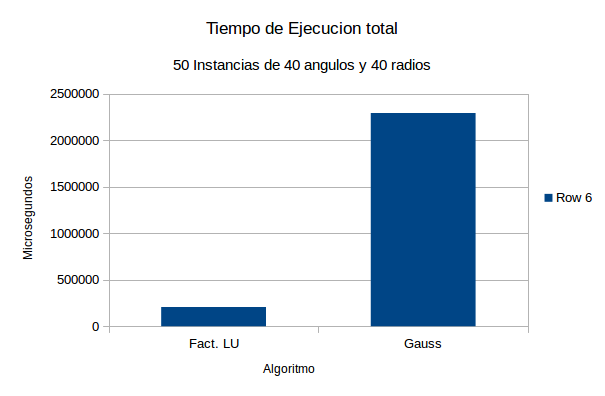
\includegraphics[scale=0.7]{experimentos2a_2b/2b4040.png}
\end{center}

 \textbf{Ratio LU/Gauss: 0.090}

  	\textbf{Comparaci\'on de Perfomance para 60 \'angulos y radios }\\
\begin{center}
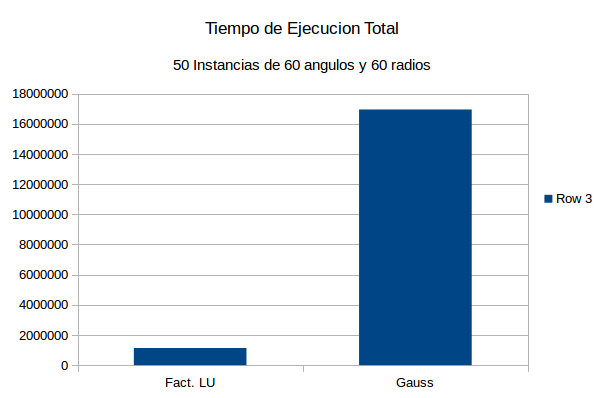
\includegraphics[scale=0.7]{experimentos2a_2b/2b6060.png}
\end{center}

 \textbf{Ratio LU/Gauss: 0.066}

Podemos notar como, a medida que mejora la discretizaci\'on, tambi\'en mejora la diferencia de perfomance de la factorizaci\'on LU por sobre Gauss, dando muestra de la diferencia de un orden polinomial de Gauss sobre LU (para la segunda instancia en adelante)

\subsubsection{Evolución estimación de la isoterma y temperatura}
Se presentarán los resultados de los experimentos en el mismo orden en que fueron planteados en la sección de desarrollo. Se realizará el análisis de los mismos en este mismo apartado.
\begin{enumerate}
	\item \begin{itemize}
				\item \textbf{Temperaturas internas y externas:} aleatorias uniformes entre $[50\dots200]$ y $[1450\dots1550]$, pero fijas entre tests.
				\item \textbf{Radio interno:} 200
				\item \textbf{Radio externo:} 400
				\item \textbf{Cantidad radios:} $[5\dots100]$
				\item \textbf{Cantidad ángulos:} 100
				\item \textbf{Isoterma buscada:} 500
			\end{itemize}
Se adjunta con el trabajo práctico un video que expone la evolución del sistema mientras se incrementa la cantidad de radios. Expondremos estáticamente algunos frames, pero es conveniente ver el video primero. Se encuentra en la misma carpeta que el pdf. (variación\_radial\_isomap.mp4, variación\_radial\_heatmap.mp4).

\vspace{0.5cm}

  	\textbf{Variación de la estimación de la isoterma entre 5 y 6 radios de discretización}\\
	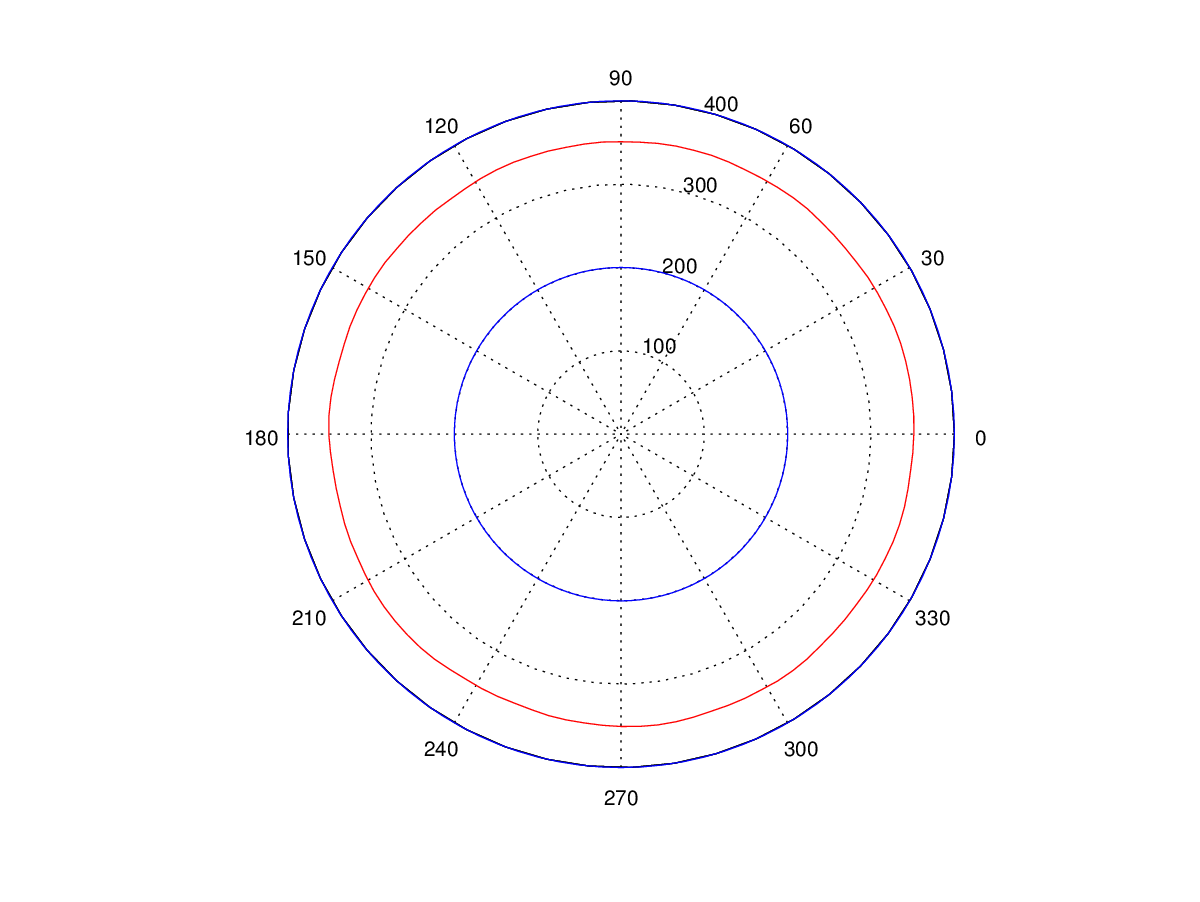
\includegraphics[scale=0.35]{experimentos1a_1b/evolucion_posicion_isoterma_temperatura/test2/test6_006_radios_inst_001_isomap.png}
	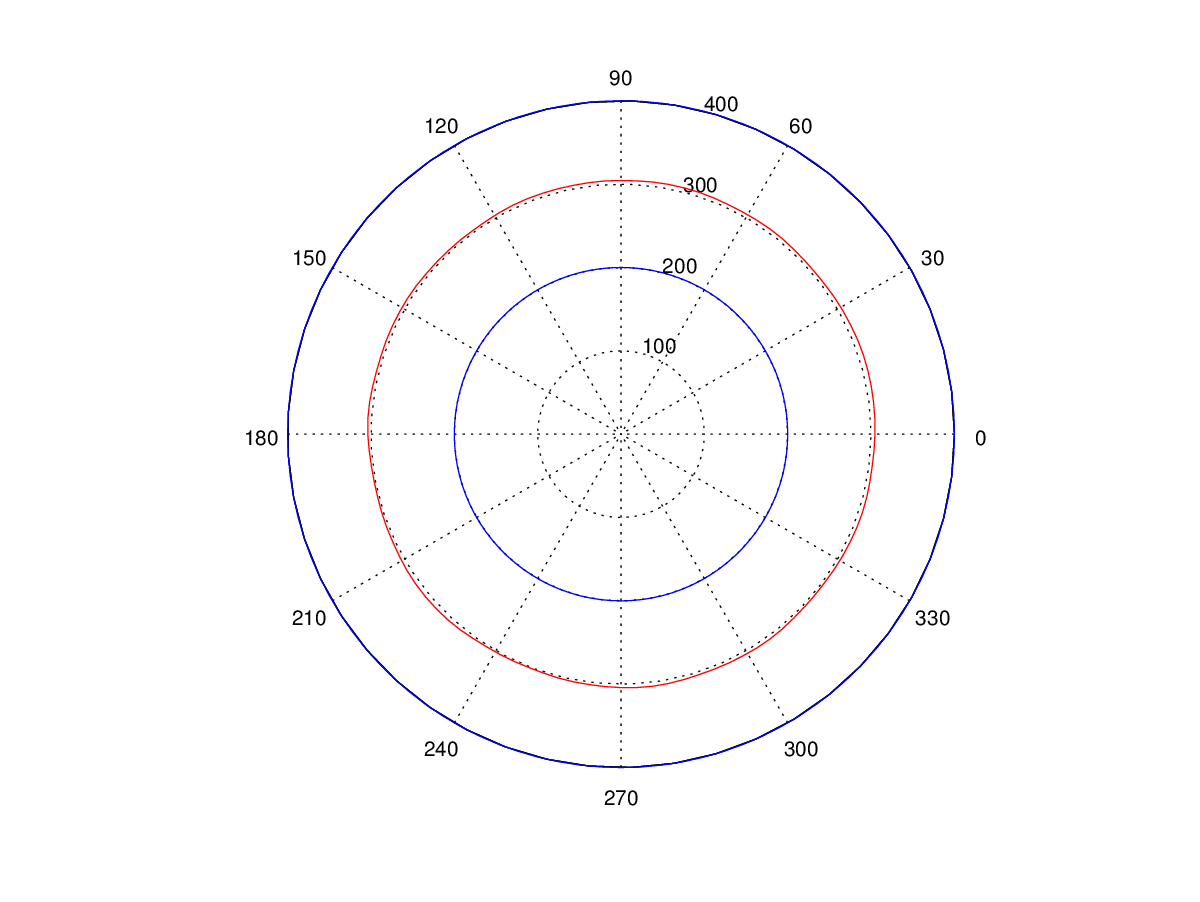
\includegraphics[scale=0.35]{experimentos1a_1b/evolucion_posicion_isoterma_temperatura/test2/test6_007_radios_inst_001_isomap.png}
	
  	\textbf{Variación de la temperatura entre 6 y 7 radios de discretización}\\
	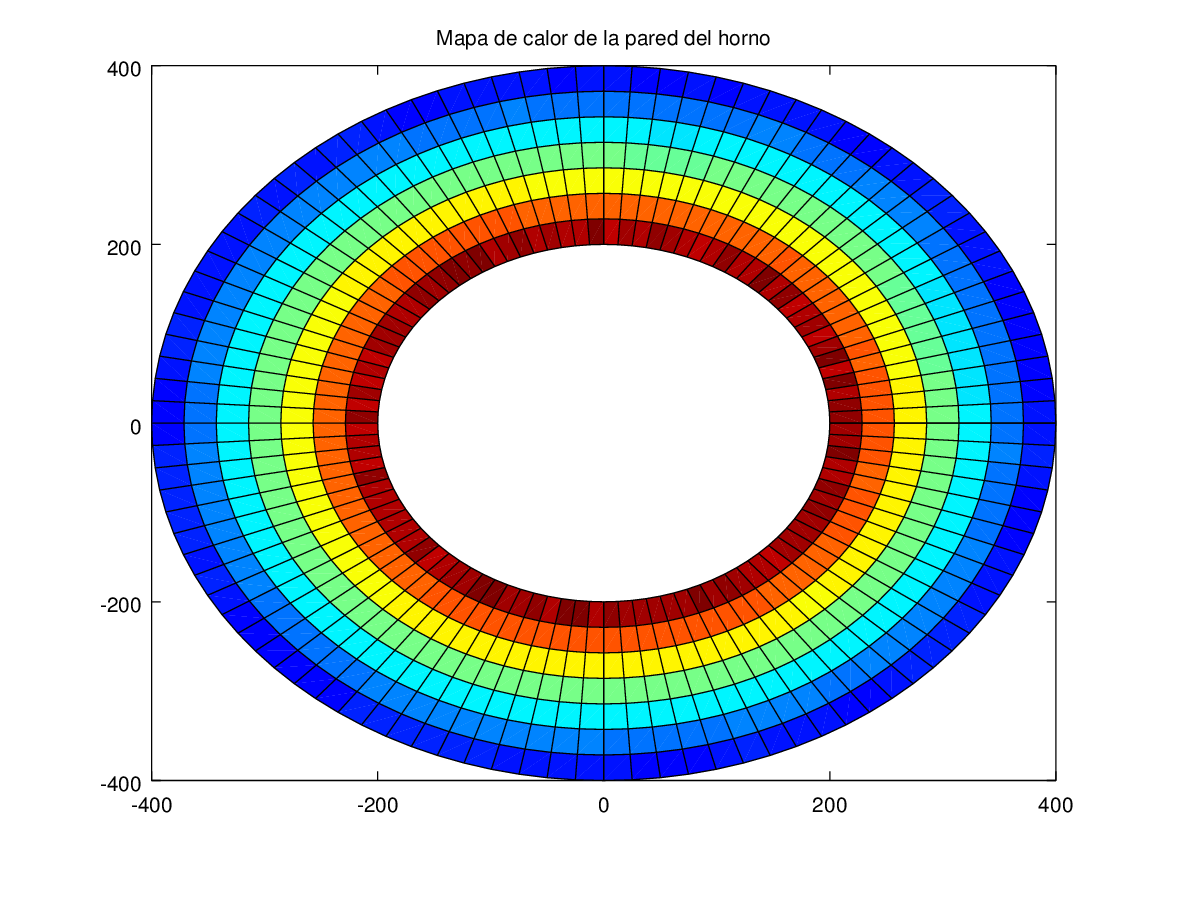
\includegraphics[scale=0.35]{experimentos1a_1b/evolucion_posicion_isoterma_temperatura/test2/test6_006_radios_inst_001_heatmap.png}
	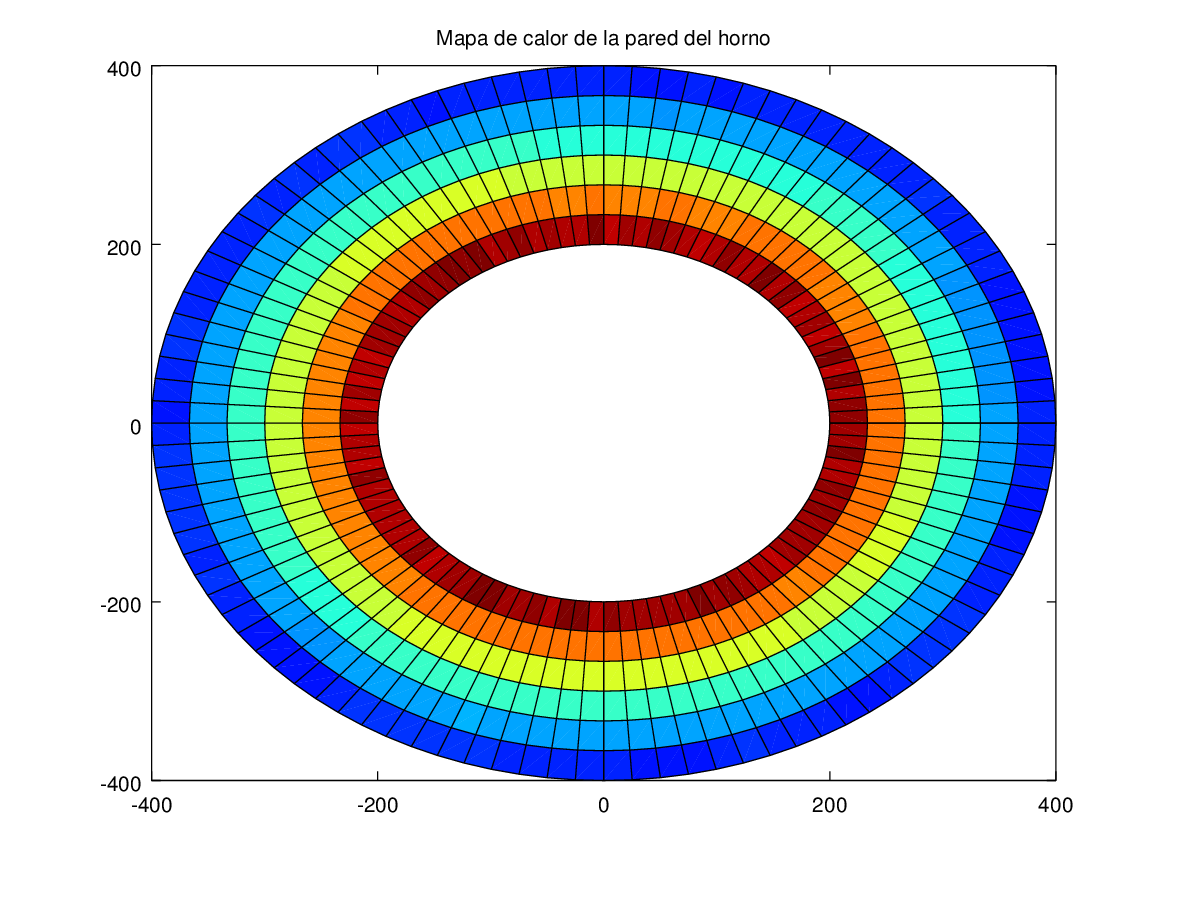
\includegraphics[scale=0.35]{experimentos1a_1b/evolucion_posicion_isoterma_temperatura/test2/test6_007_radios_inst_001_heatmap.png}

 	\textbf{Variación de la estimación de la isoterma entre 99 y 100 radios de discretización}\\
	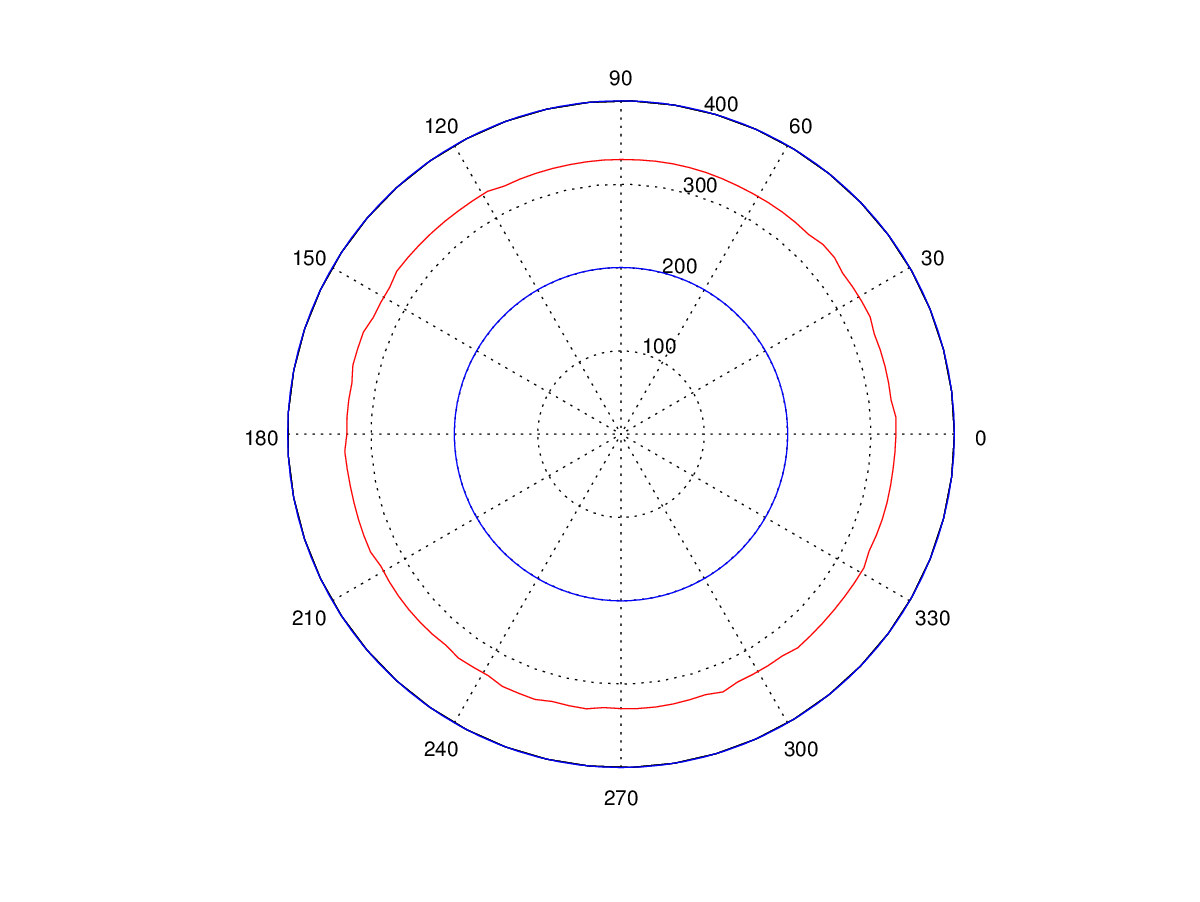
\includegraphics[scale=0.35]{experimentos1a_1b/evolucion_posicion_isoterma_temperatura/test2/test6_099_radios_inst_001_isomap.png}
	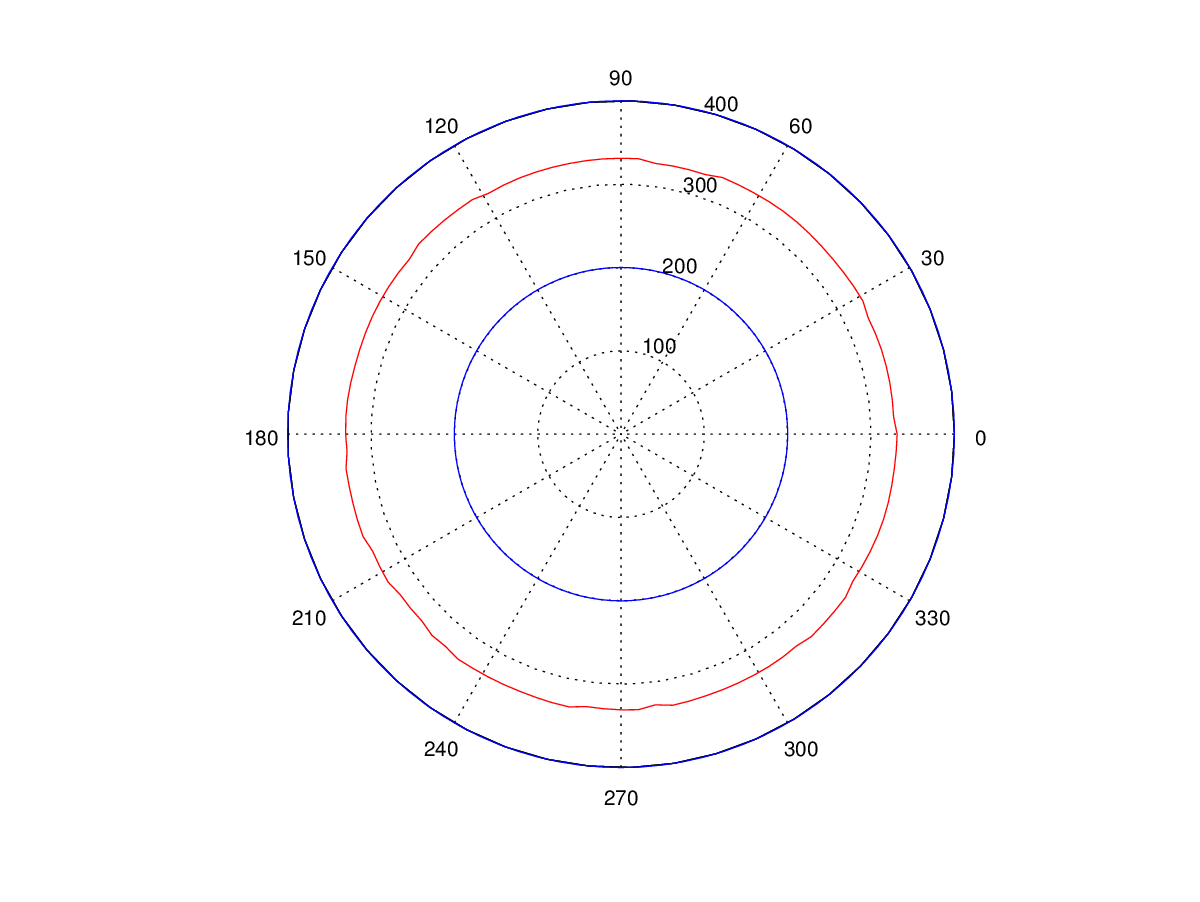
\includegraphics[scale=0.35]{experimentos1a_1b/evolucion_posicion_isoterma_temperatura/test2/test6_100_radios_inst_001_isomap.png}
	
	\textbf{Variación de la temperatura entre 99 y 100 radios de discretización}\\
	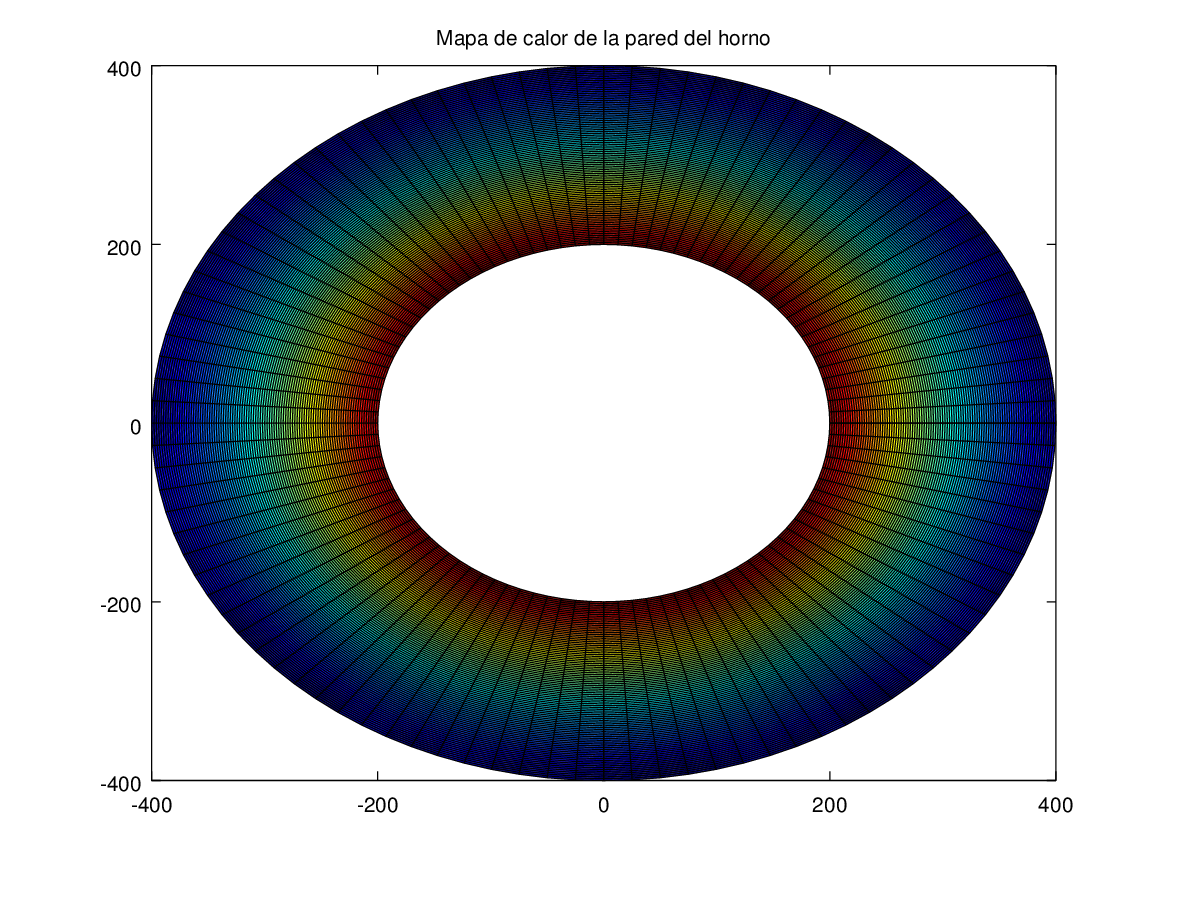
\includegraphics[scale=0.35]{experimentos1a_1b/evolucion_posicion_isoterma_temperatura/test2/test6_099_radios_inst_001_heatmap.png}
	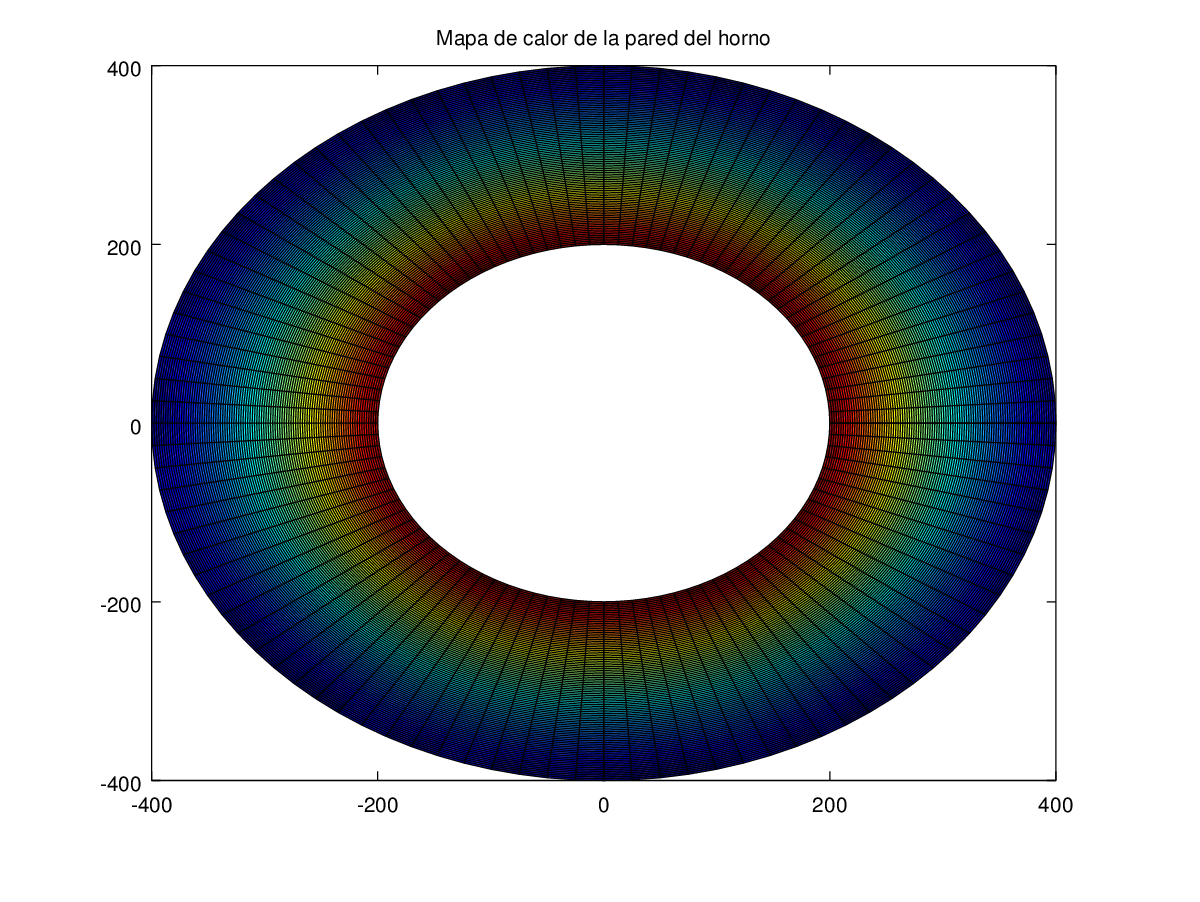
\includegraphics[scale=0.35]{experimentos1a_1b/evolucion_posicion_isoterma_temperatura/test2/test6_100_radios_inst_001_heatmap.png}

\vspace{0.5cm}

Se observa es que a medida que se aumenta la cantidad de radios de la discretización, la variación radial de la curva de la isoterma disminuye entre tests, es decir, se hace más fina la estimación, de forma tal que entre $i$ e $i+1$ radios la diferencia de la posición de la isoterma es menor a medida que $i$ crece. Para ver mejor esto se graficaron, para cada test de $i$ cantidad de radios de la discretización, el máximo y el promedio radial de la isoterma.

	\textbf{Evolución de la variación radial de la isoterma con cantidad creciente de radios}\\
	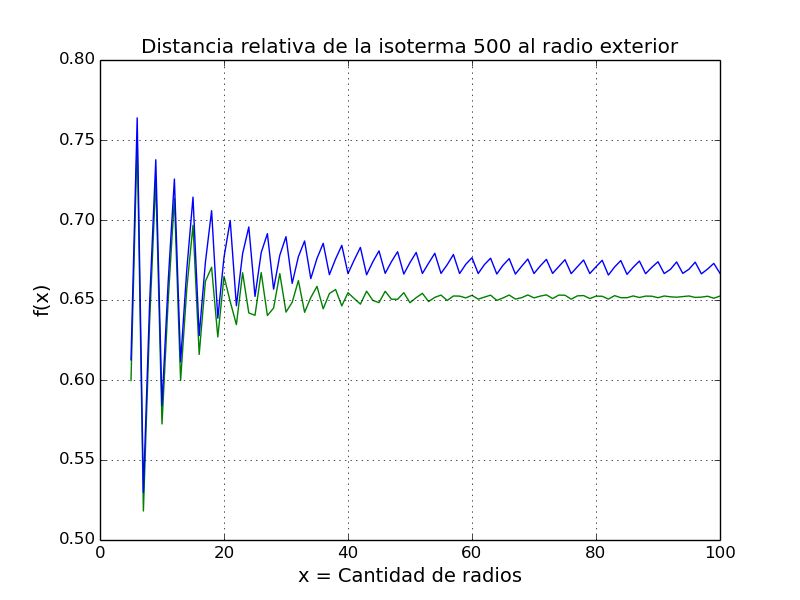
\includegraphics[scale=0.5]{experimentos1a_1b/evolucion_estimacion_seguridad_isoterma/100ang_5to100radios.png}\\

	\item \begin{itemize}
					\item \textbf{Temperaturas internas y externas:} constantes, 100 y 1500. Esto es para que tenga la misma solución cada test del experimento.
					\item \textbf{Radio interno:} 200
					\item \textbf{Radio externo:} 400
					\item \textbf{Cantidad radios:} 50
					\item \textbf{Cantidad ángulos:} $[5\dots50]$
					\item \textbf{Isoterma buscada:} 500
				\end{itemize}
	Se adjunta con el trabajo práctico un video que expone la evolución del sistema mientras se incrementa la cantidad de radios. Expondremos estáticamente algunos frames, pero es conveniente ver el video primero. Se encuentra en la misma carpeta que el pdf. (variación\_angular\_isomap.mp4, variación\_angular\_heatmap.mp4).

	\vspace{0.5cm}
	  	\textbf{Variación de la estimación de la isoterma entre 5 y 6 ángulos de discretización}\\
		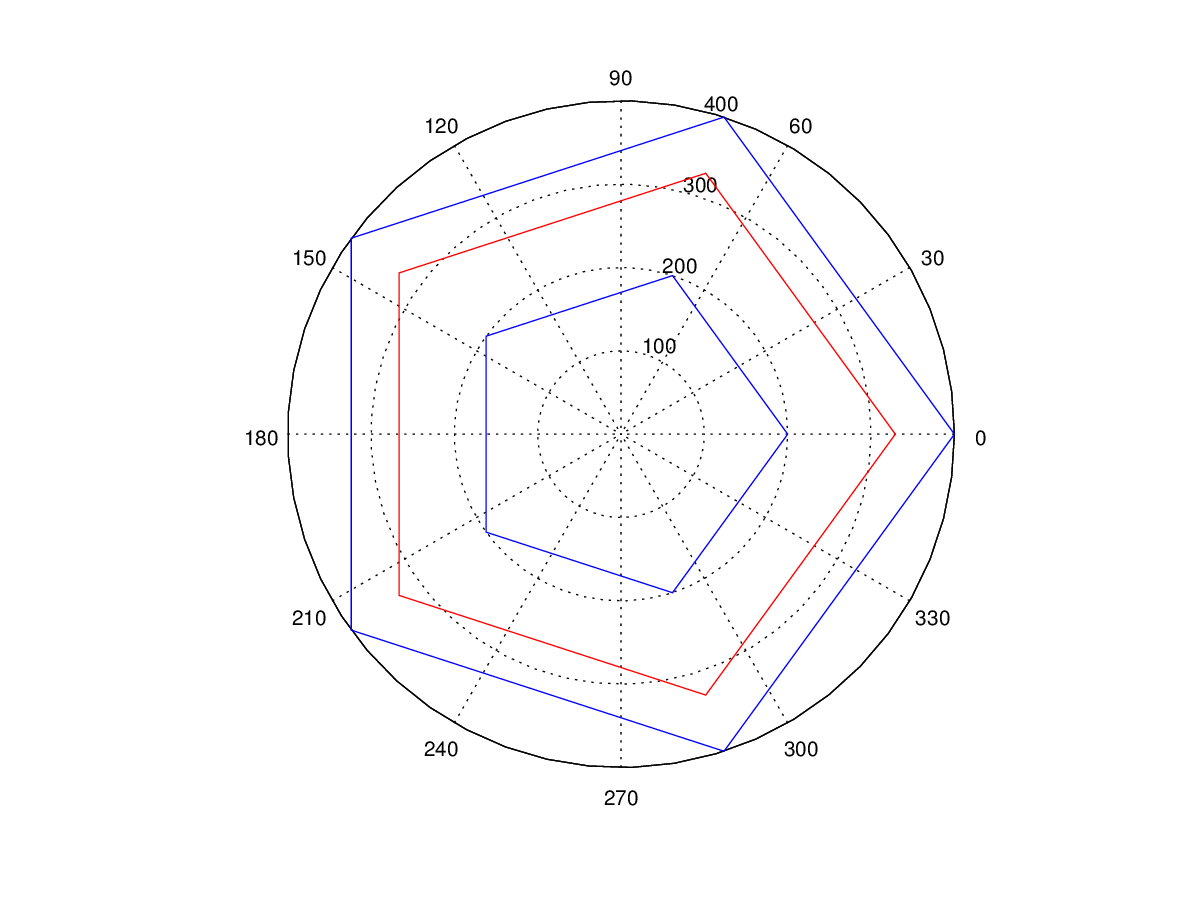
\includegraphics[scale=0.35]{experimentos1a_1b/evolucion_posicion_isoterma_temperatura/variacion_angulos_radio_fijo_se_suaviza_isoterma/test10_050_radios_005_angulos_inst_001_isomap.png}
		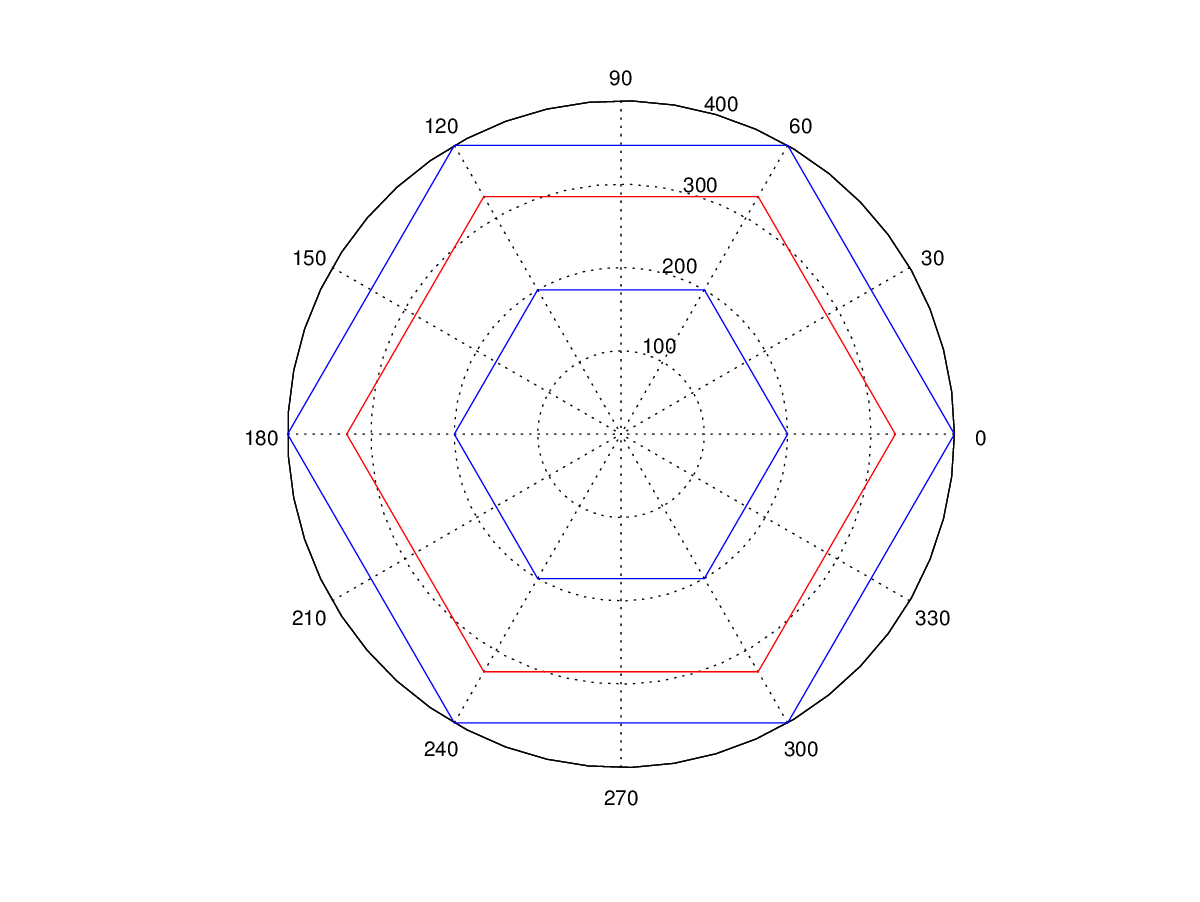
\includegraphics[scale=0.35]{experimentos1a_1b/evolucion_posicion_isoterma_temperatura/variacion_angulos_radio_fijo_se_suaviza_isoterma/test10_050_radios_006_angulos_inst_001_isomap.png}

	  	\textbf{Variación de la temperatura entre 5 y 6 ángulos de discretización}\\
	  	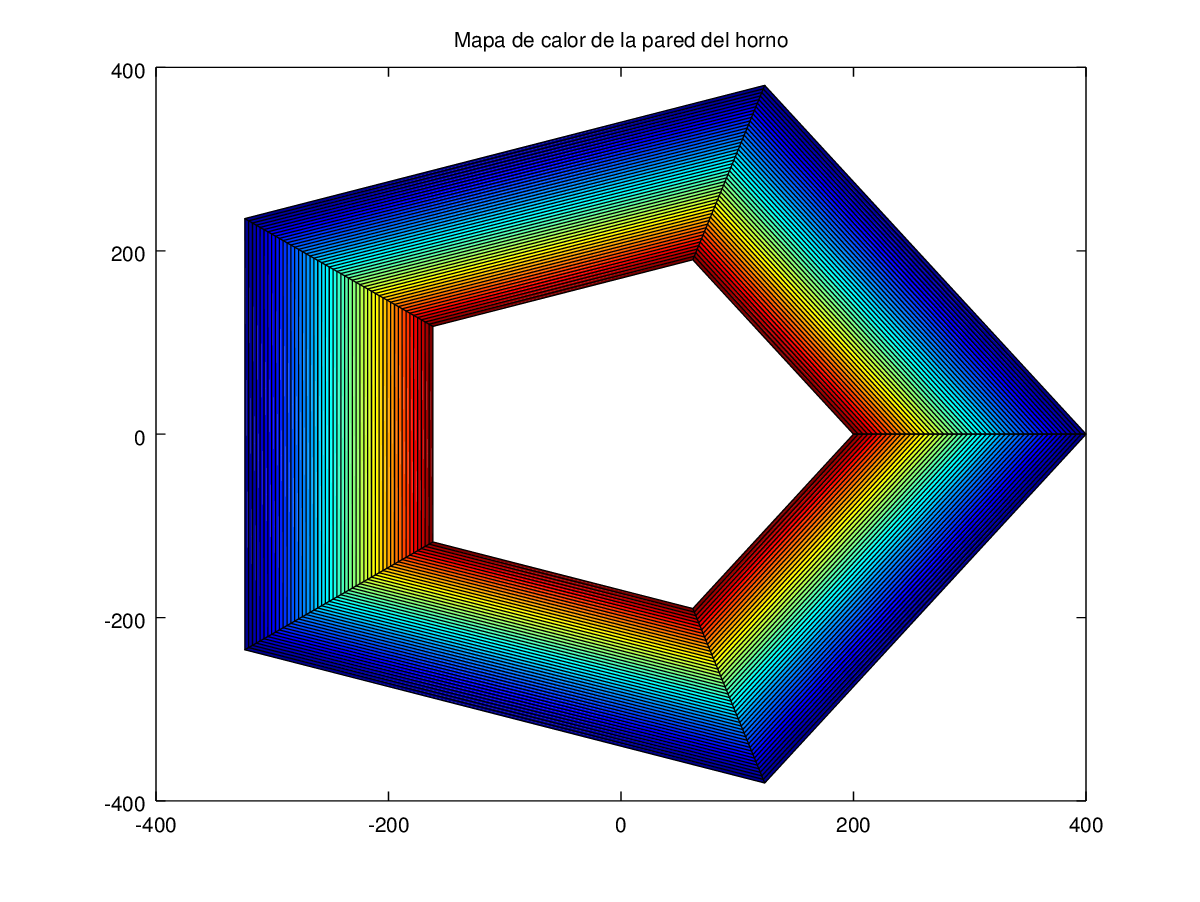
\includegraphics[scale=0.35]{experimentos1a_1b/evolucion_posicion_isoterma_temperatura/variacion_angulos_radio_fijo_se_suaviza_isoterma/test10_050_radios_005_angulos_inst_001_heatmap.png}
		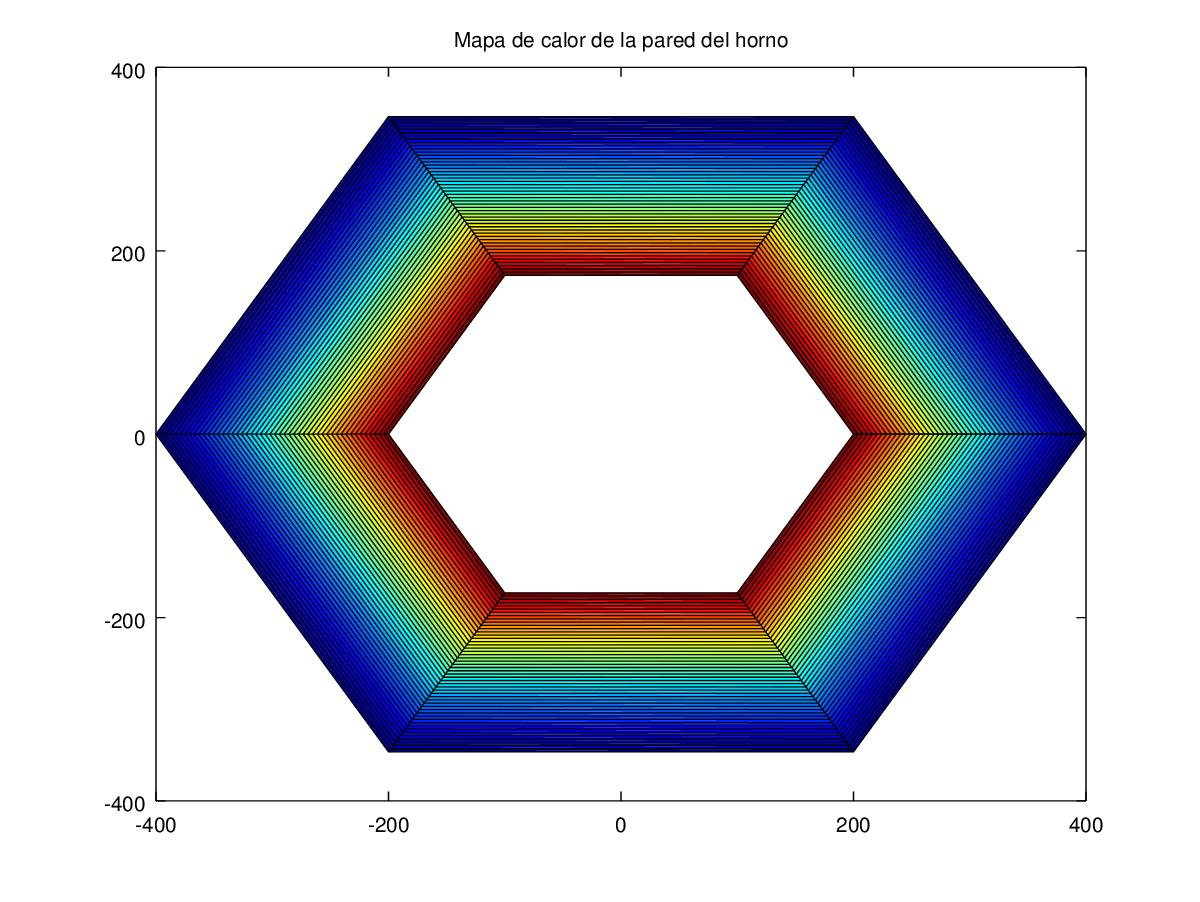
\includegraphics[scale=0.35]{experimentos1a_1b/evolucion_posicion_isoterma_temperatura/variacion_angulos_radio_fijo_se_suaviza_isoterma/test10_050_radios_006_angulos_inst_001_heatmap.png}	  	

	  	\textbf{Variación de la estimación de la isoterma entre 49 y 50 ángulos de discretización}\\
		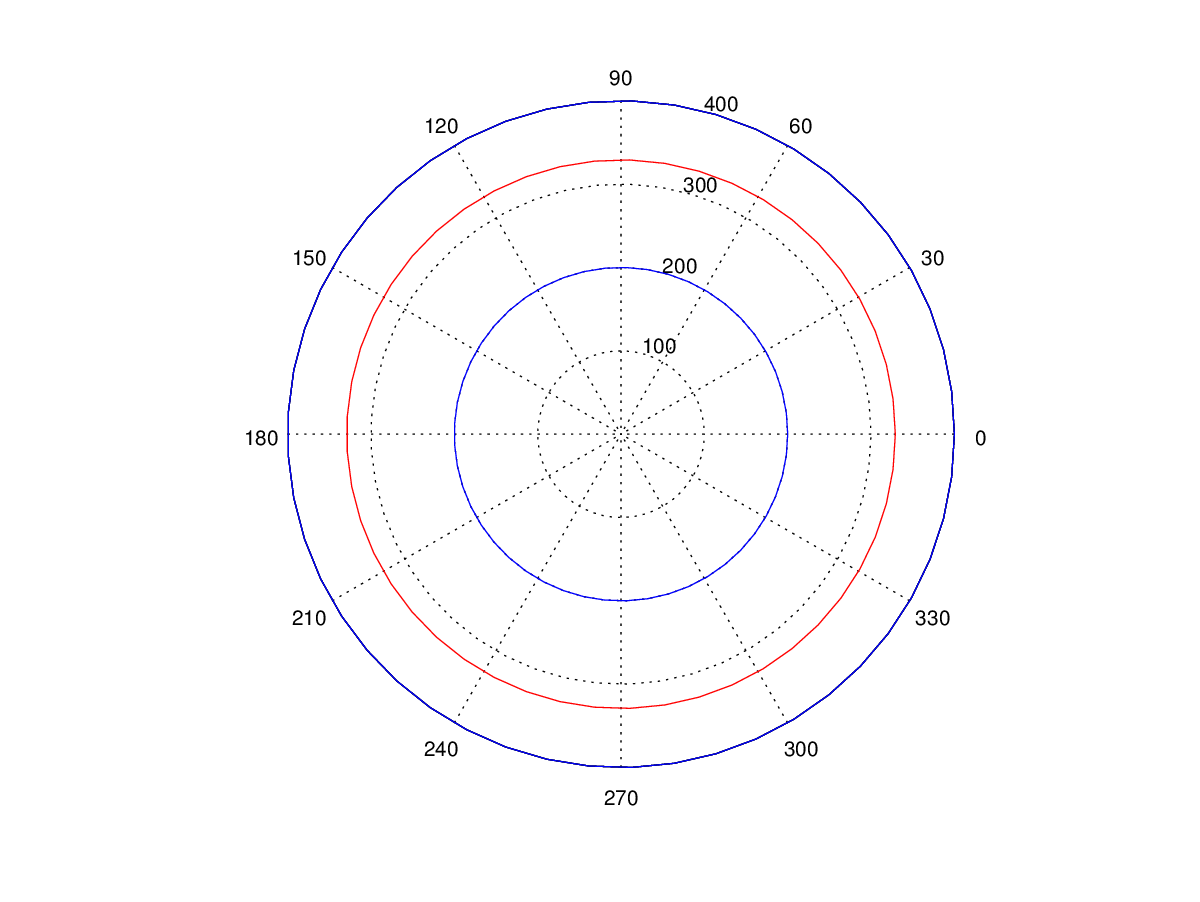
\includegraphics[scale=0.35]{experimentos1a_1b/evolucion_posicion_isoterma_temperatura/variacion_angulos_radio_fijo_se_suaviza_isoterma/test10_050_radios_049_angulos_inst_001_isomap.png}
		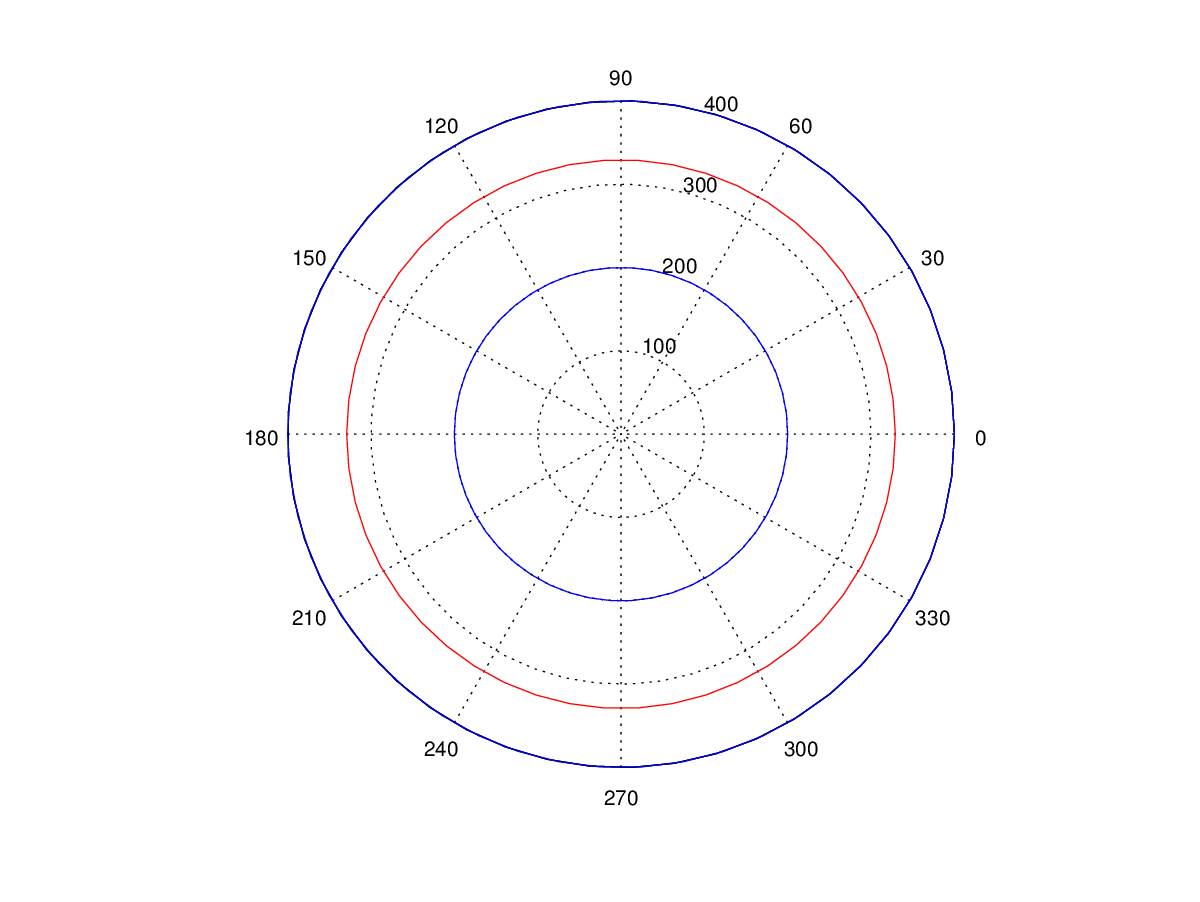
\includegraphics[scale=0.35]{experimentos1a_1b/evolucion_posicion_isoterma_temperatura/variacion_angulos_radio_fijo_se_suaviza_isoterma/test10_050_radios_050_angulos_inst_001_isomap.png}

		\textbf{Variación de la temperatura entre 49 y 50 ángulos de discretización}\\
	  	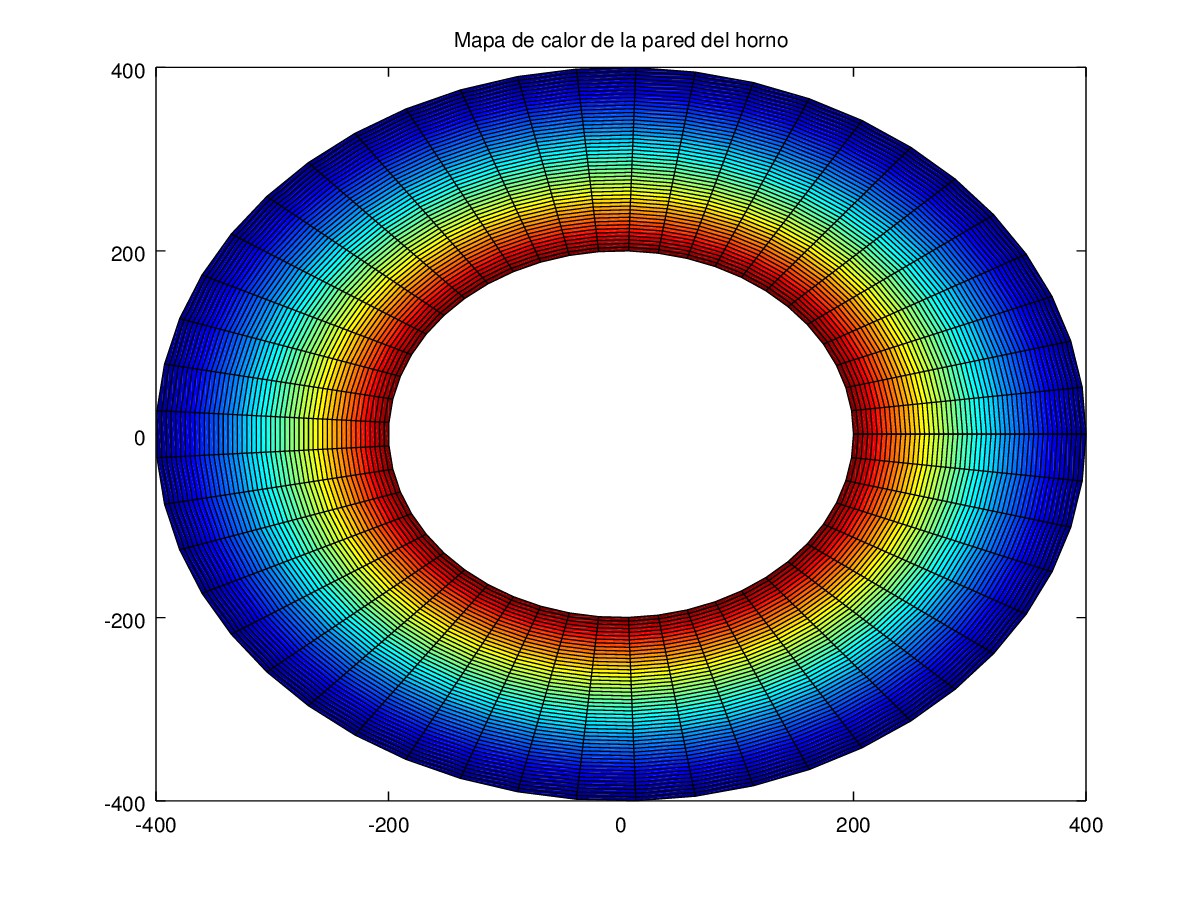
\includegraphics[scale=0.35]{experimentos1a_1b/evolucion_posicion_isoterma_temperatura/variacion_angulos_radio_fijo_se_suaviza_isoterma/test10_050_radios_049_angulos_inst_001_heatmap.png}
		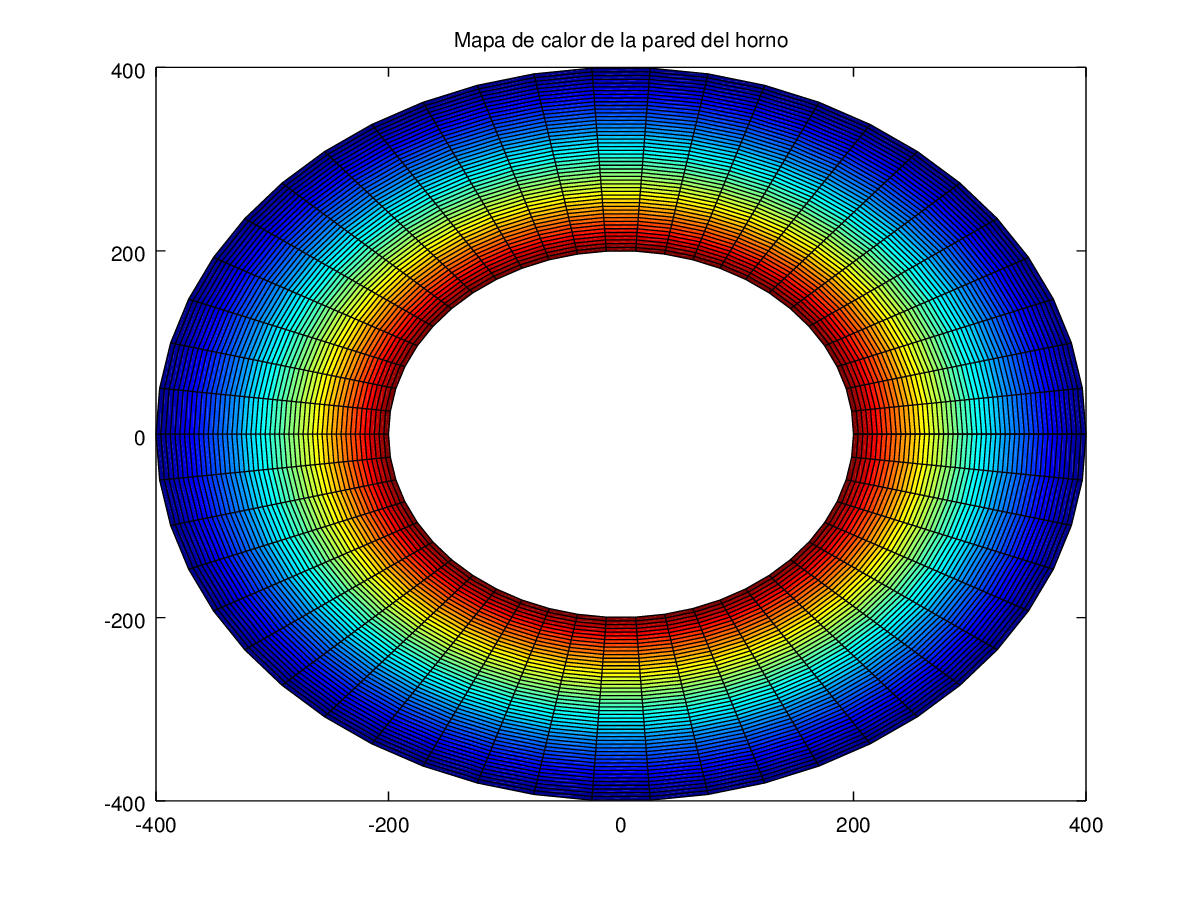
\includegraphics[scale=0.35]{experimentos1a_1b/evolucion_posicion_isoterma_temperatura/variacion_angulos_radio_fijo_se_suaviza_isoterma/test10_050_radios_050_angulos_inst_001_heatmap.png}

\vspace{0.5cm}

Aquí el radio es el mismo, pero se gana en precisión al tener más ángulos por no tener que linealizar la posición de la isoterma angularmente. Nuevamente, la posición entre dos tests consecutivos se estabiliza al aumentar la cantidad de ángulos. Tambien se observa que al cambiar el $\Delta_\theta$ los ángulos entre tests consecutivos no son los mismos.

	\item \begin{itemize}
						\item \textbf{Temperaturas internas y externas:} constantes, 100 y 1500. Esto es para que tenga la misma solución cada test del experimento.
						\item \textbf{Radio interno:} 200
						\item \textbf{Radio externo:} 400
						\item \textbf{Cantidad radios:} $[15\dots60]$
						\item \textbf{Cantidad ángulos:} $[15\dots60]$
						\item \textbf{Isoterma buscada:} 500
					\end{itemize}
	Se adjunta con el trabajo práctico un video que expone la evolución del sistema mientras se incrementa la cantidad de radios. Expondremos estáticamente algunos frames, pero es conveniente ver el video primero. Se encuentra en la misma carpeta que el pdf. (variación\_doble\_isomap.mp4, variación\_doble\_heatmap.mp4).

	\vspace{0.5cm}
	  	\textbf{Variación de la estimación de la isoterma entre 15 y 16 radios, ángulos de discretización}\\
		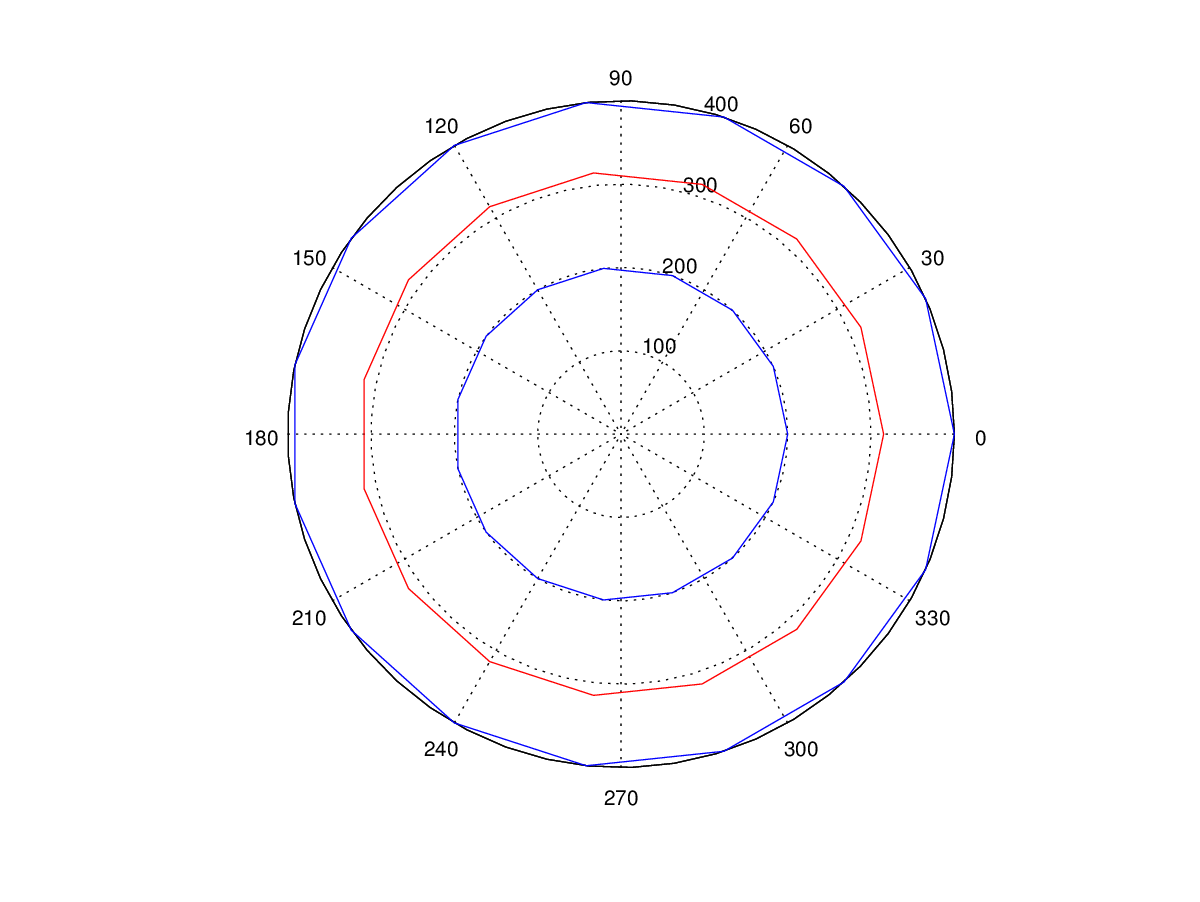
\includegraphics[scale=0.35]{experimentos1a_1b/evolucion_posicion_isoterma_temperatura/variacion_radios_angulos_se_reduce_diferencia_radial/test11_testord_001_inst_001_isomap.png}
		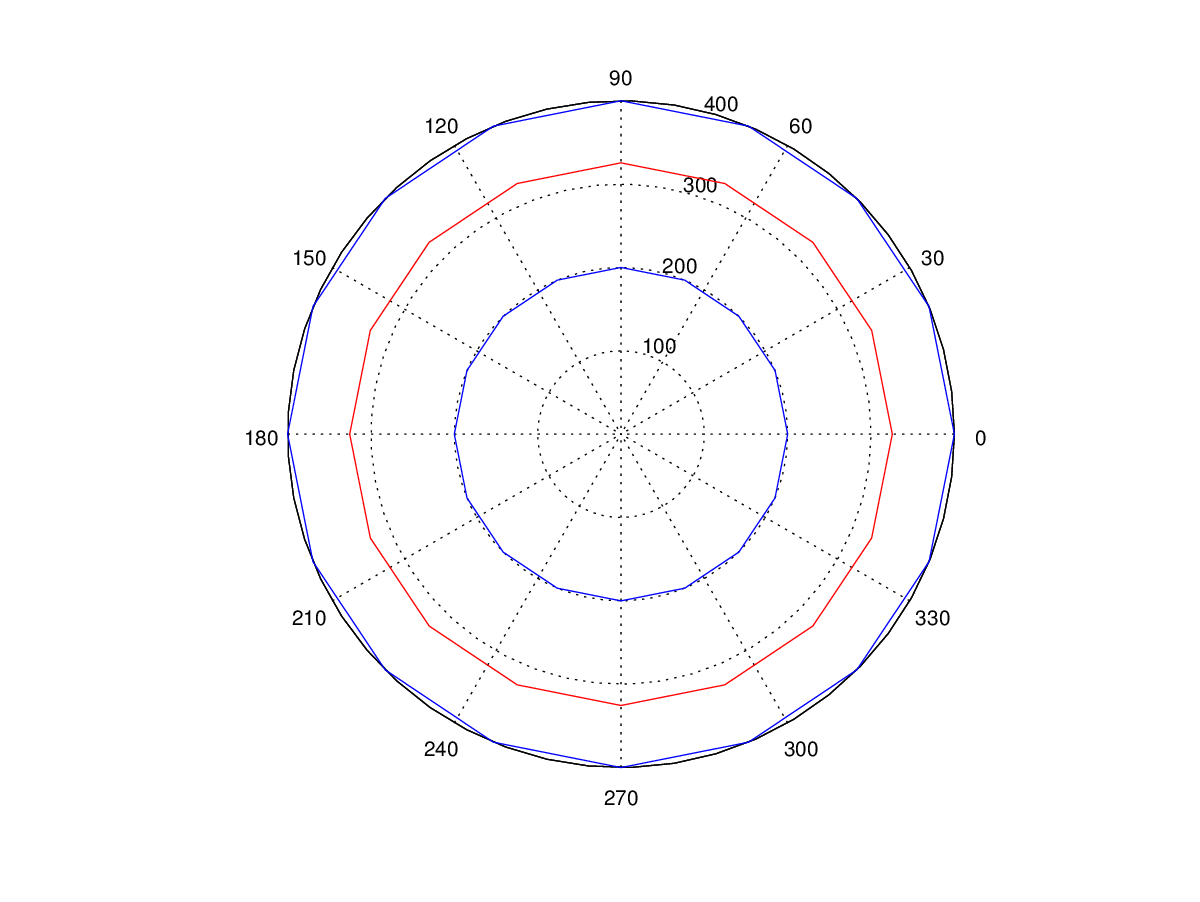
\includegraphics[scale=0.35]{experimentos1a_1b/evolucion_posicion_isoterma_temperatura/variacion_radios_angulos_se_reduce_diferencia_radial/test11_testord_002_inst_001_isomap.png}

	  	\textbf{Variación de la temperatura entre 59 y 60 radios, ángulos de discretización}\\
	  	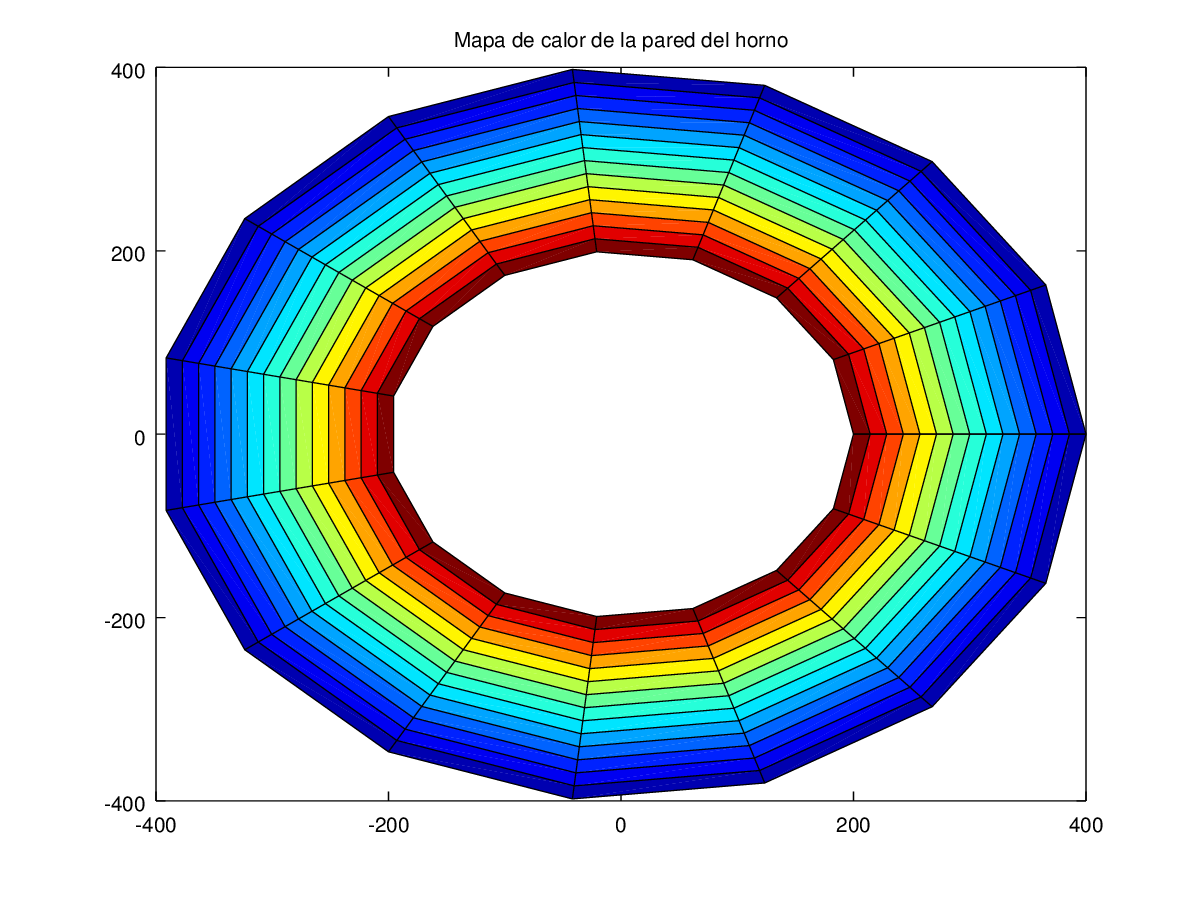
\includegraphics[scale=0.35]{experimentos1a_1b/evolucion_posicion_isoterma_temperatura/variacion_radios_angulos_se_reduce_diferencia_radial/test11_testord_001_inst_001_heatmap.png}
		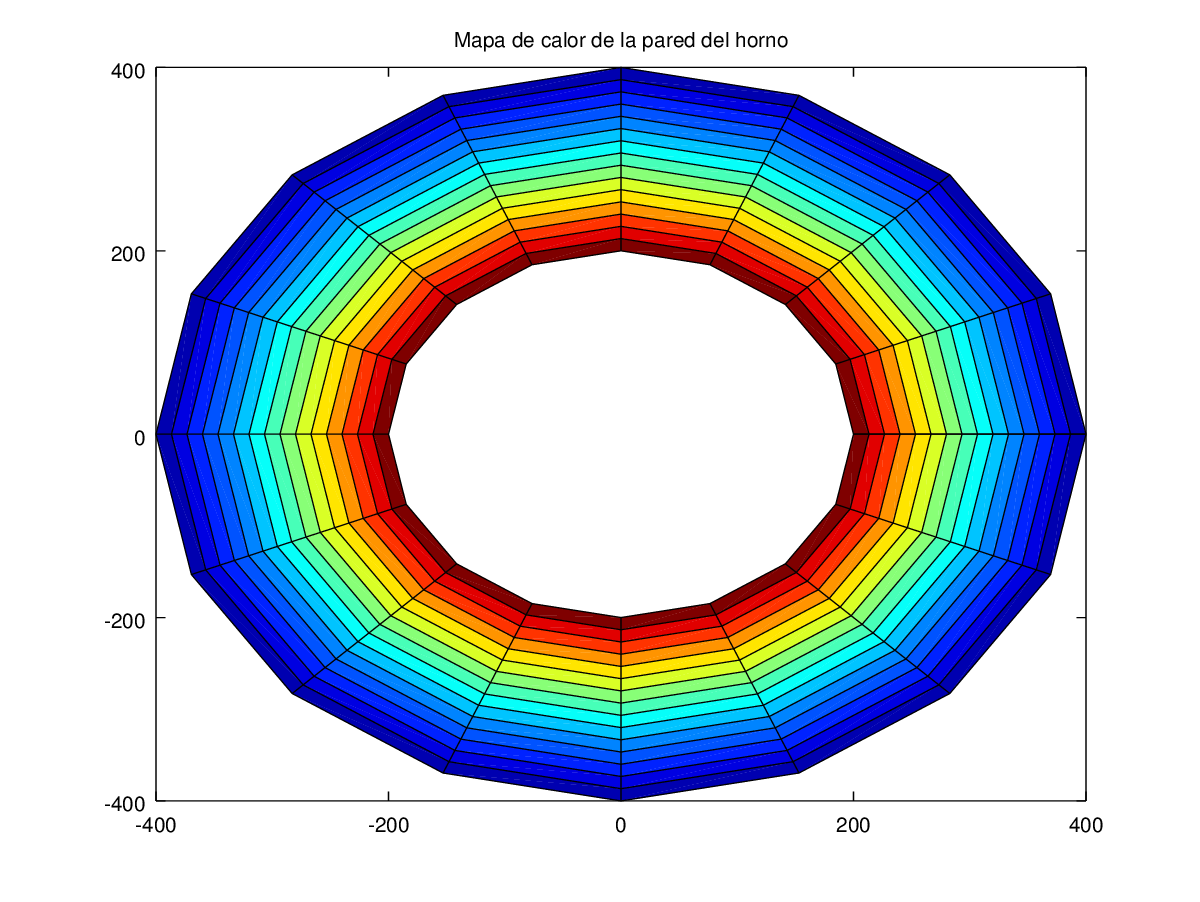
\includegraphics[scale=0.35]{experimentos1a_1b/evolucion_posicion_isoterma_temperatura/variacion_radios_angulos_se_reduce_diferencia_radial/test11_testord_002_inst_001_heatmap.png}

	  	\textbf{Variación de la estimación de la isoterma entre 15 y 16 radios, ángulos de discretización}\\
		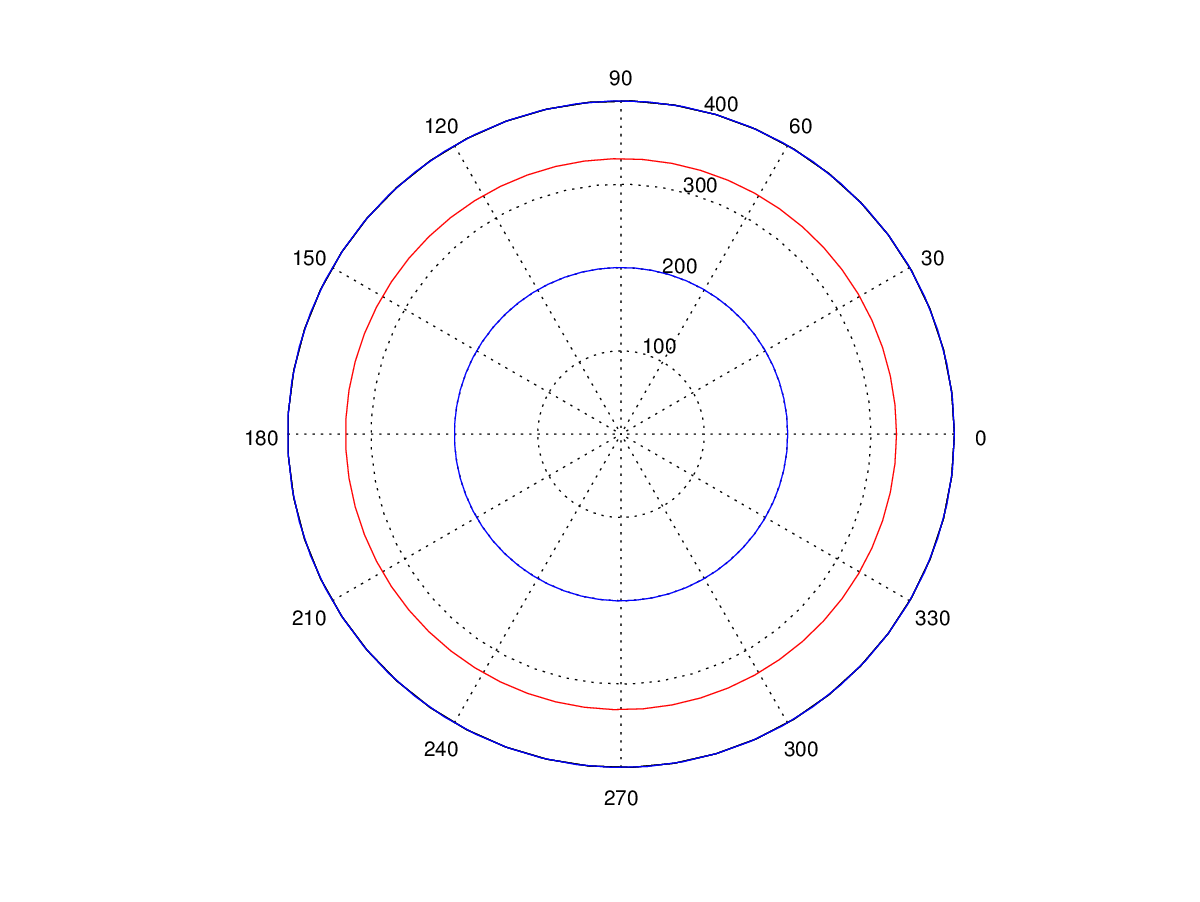
\includegraphics[scale=0.35]{experimentos1a_1b/evolucion_posicion_isoterma_temperatura/variacion_radios_angulos_se_reduce_diferencia_radial/test11_testord_045_inst_001_isomap.png}
		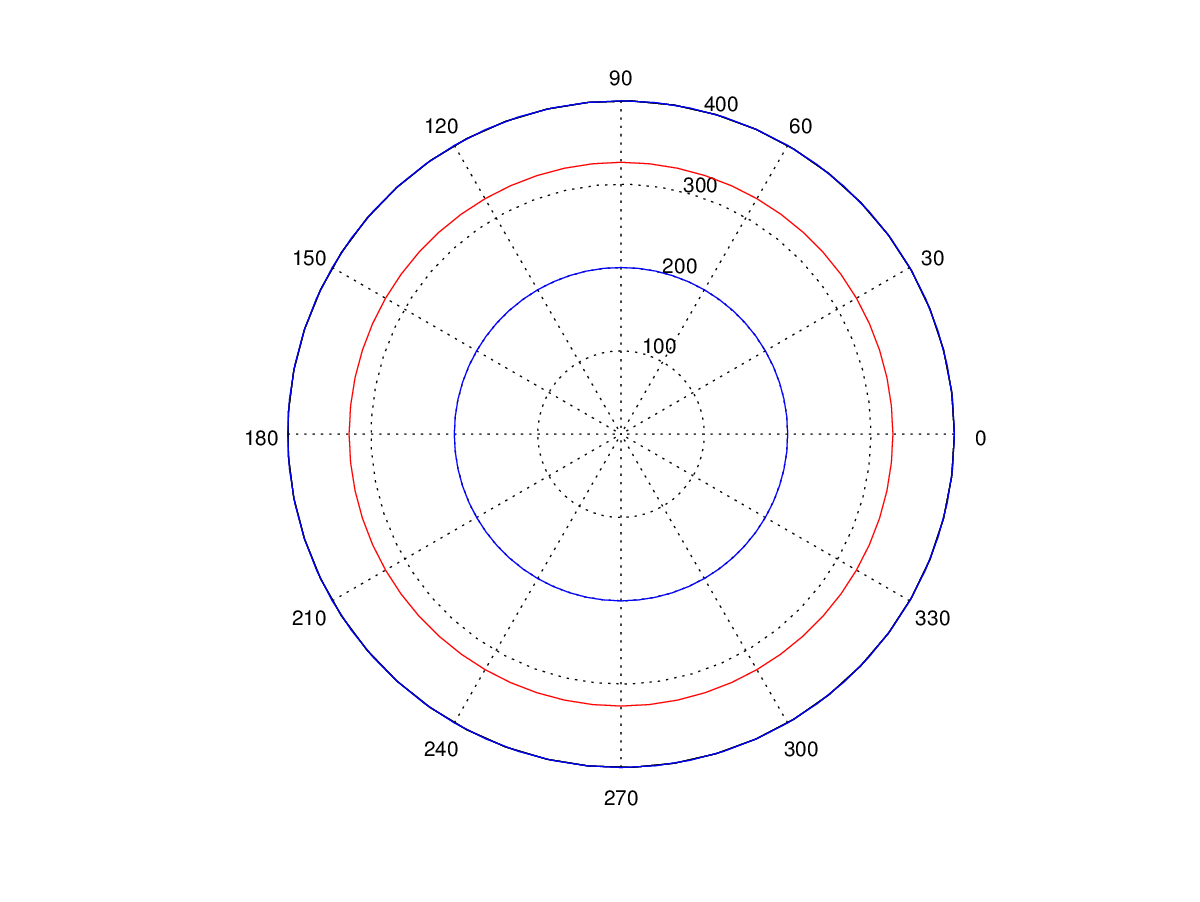
\includegraphics[scale=0.35]{experimentos1a_1b/evolucion_posicion_isoterma_temperatura/variacion_radios_angulos_se_reduce_diferencia_radial/test11_testord_046_inst_001_isomap.png}

		\textbf{Variación de la temperatura entre 59 y 60 radios, ángulos de discretización}\\
	  	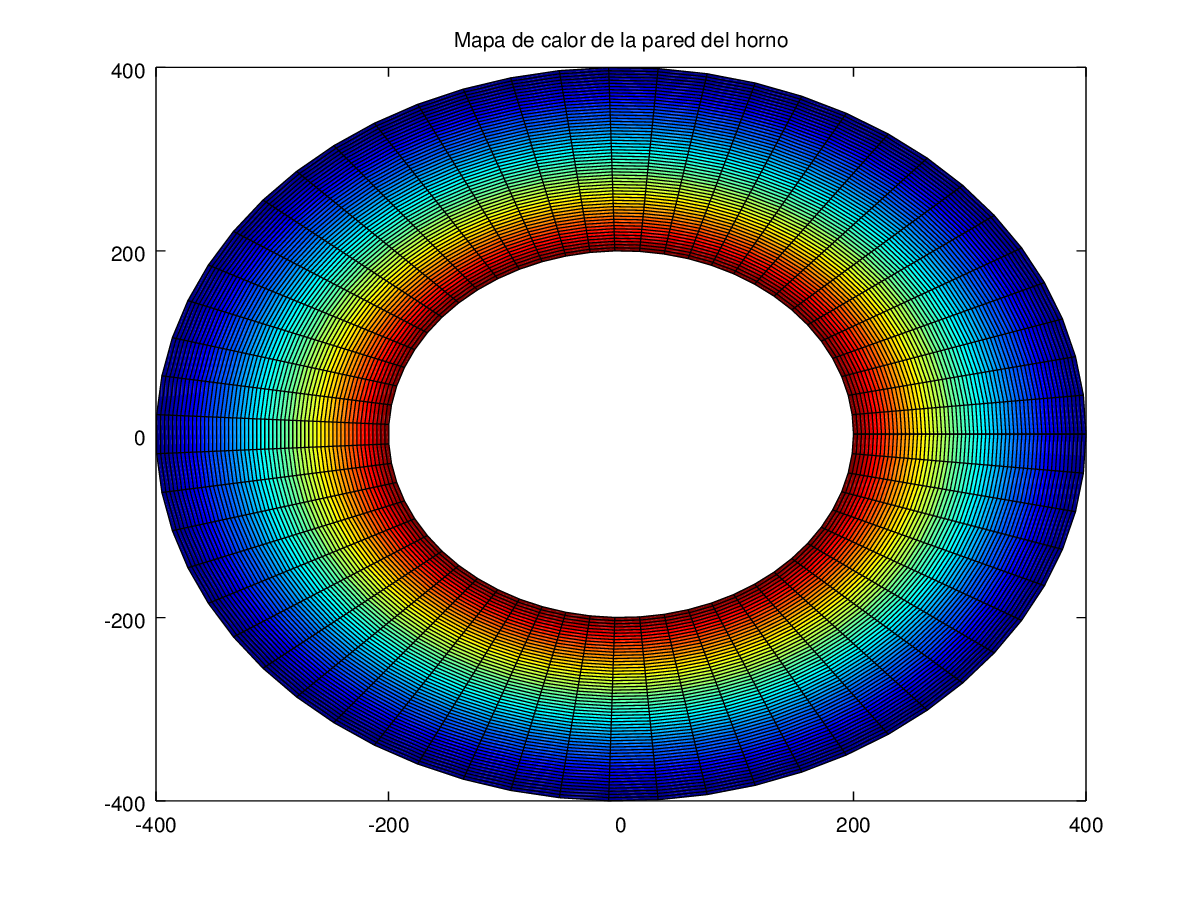
\includegraphics[scale=0.35]{experimentos1a_1b/evolucion_posicion_isoterma_temperatura/variacion_radios_angulos_se_reduce_diferencia_radial/test11_testord_045_inst_001_heatmap.png}
		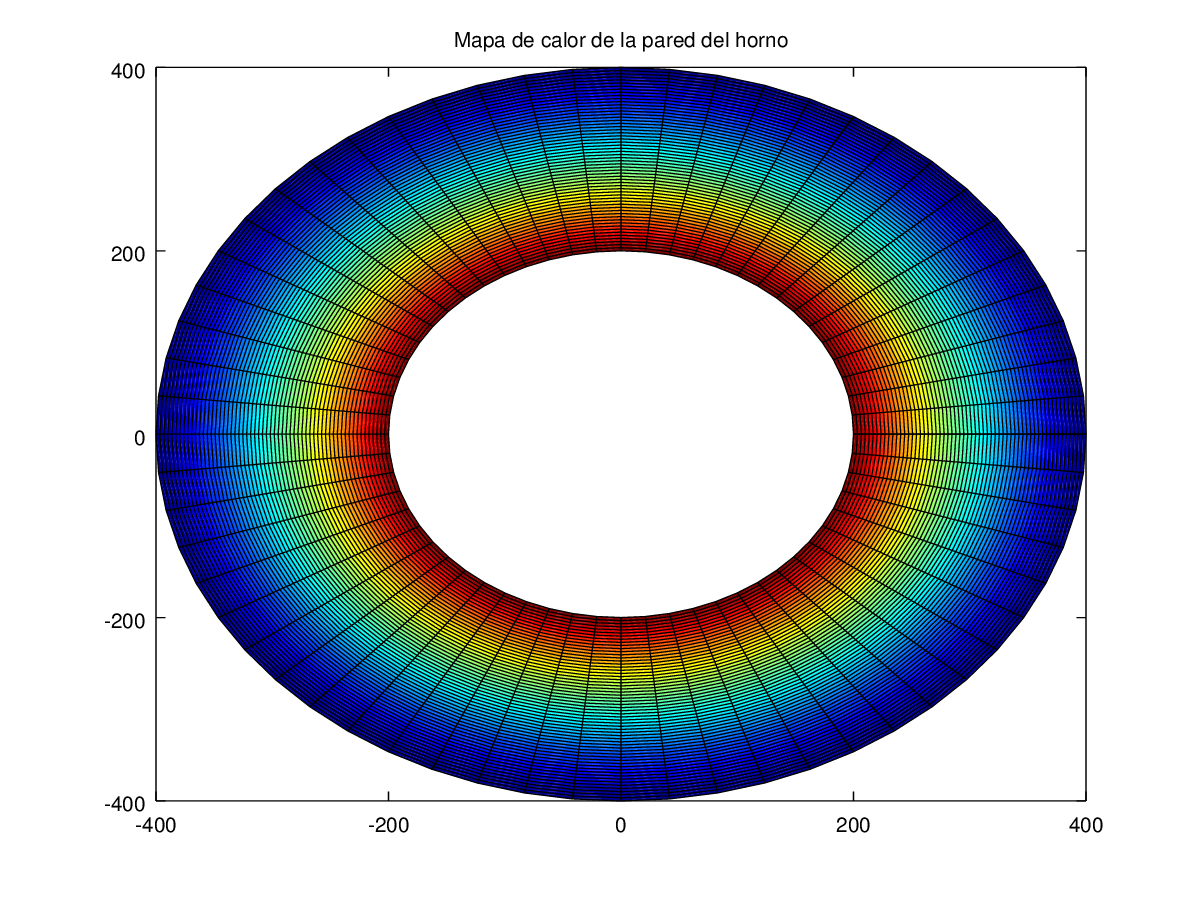
\includegraphics[scale=0.35]{experimentos1a_1b/evolucion_posicion_isoterma_temperatura/variacion_radios_angulos_se_reduce_diferencia_radial/test11_testord_046_inst_001_heatmap.png}

\vspace{0.5cm}

En este último ejemplo ocurren ambos fenomenos al mismo tiempo, hay una variación radial menor a medida que crecen los radios y la curva se suaviza al aumentar los ángulos.

\end{enumerate}

\vspace{0.5cm}

Efectivamente, podemos concluir que mientras más fina sea la discretización, se obtendrán resultados más \texttt{estables y confiables} acerca de la estimación. Uno de los motivos es porque habrá menos puntos para interpolar en la posición de la isoterma y el otro porque se tiene más informacion de la temperatura de la pared del horno.

\subsubsection{Estimación de estabilidad de la pared del horno}
Para este experimento utilizaremos discretizaciones finas, ya vimos en los experimentos anteriores que esto provee mayor confiabilidad en las estimaciones, para discretizaciones más gruesas las estimaciones de seguridad serán menos exactas.
\vspace{0.5cm}

\begin{itemize}
	\item \textbf{Temperaturas internas:} $[200, 500, 750]$
	\item \textbf{Temperaturas externas:} $[1450\dots1550]$ aleatorias uniformes.
	\item \textbf{Radio interno:} 200
	\item \textbf{Radio externo:} 400
	\item \textbf{Cantidad radios:} 30
	\item \textbf{Cantidad ángulos:} 30
	\item \textbf{Isoterma buscada:} 500
\end{itemize}

	\textbf{Temperaturas externas: } 200\\
	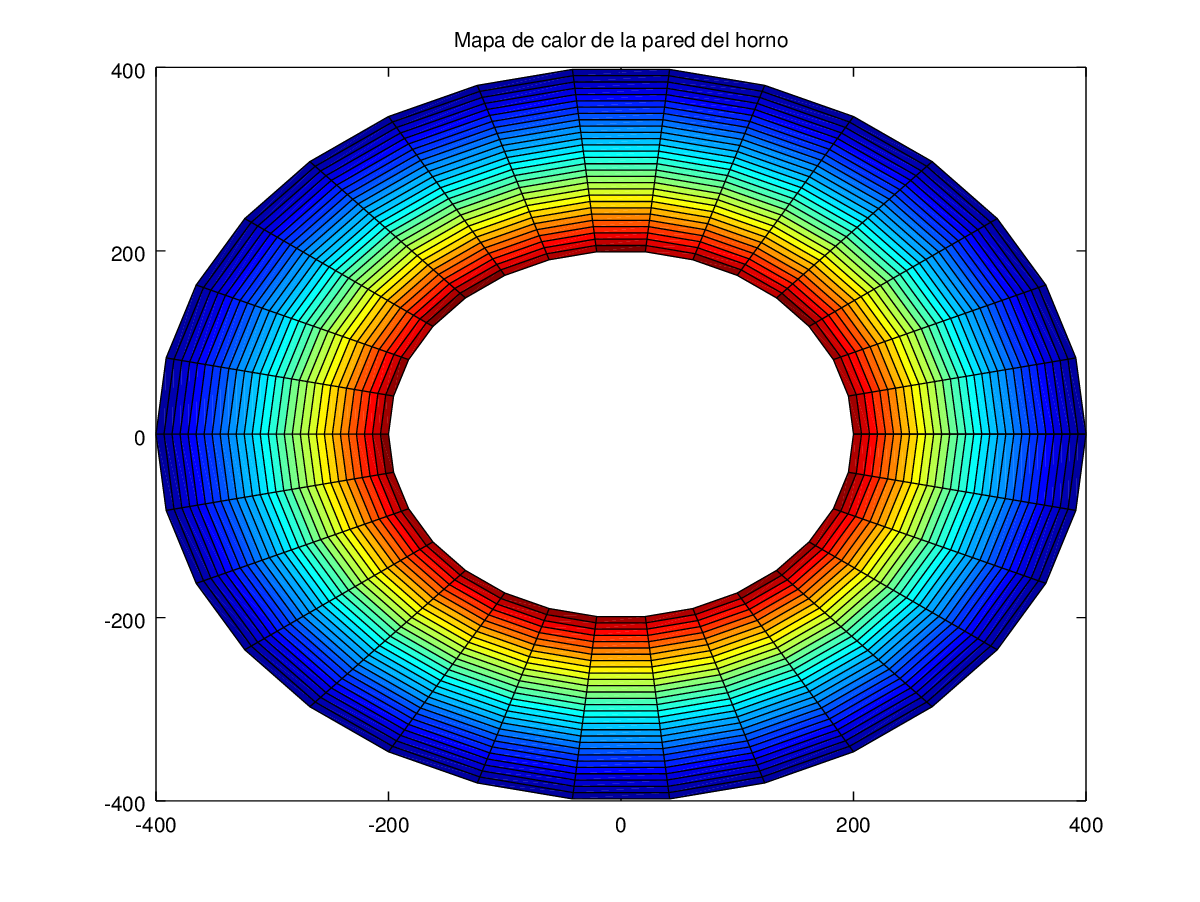
\includegraphics[scale=0.35]{experimentos1a_1b/evolucion_isoterma_cambios_temperatura_varias_discretizaciones/test21_030_radios_030_angulos_inst_001_heatmap.png}
	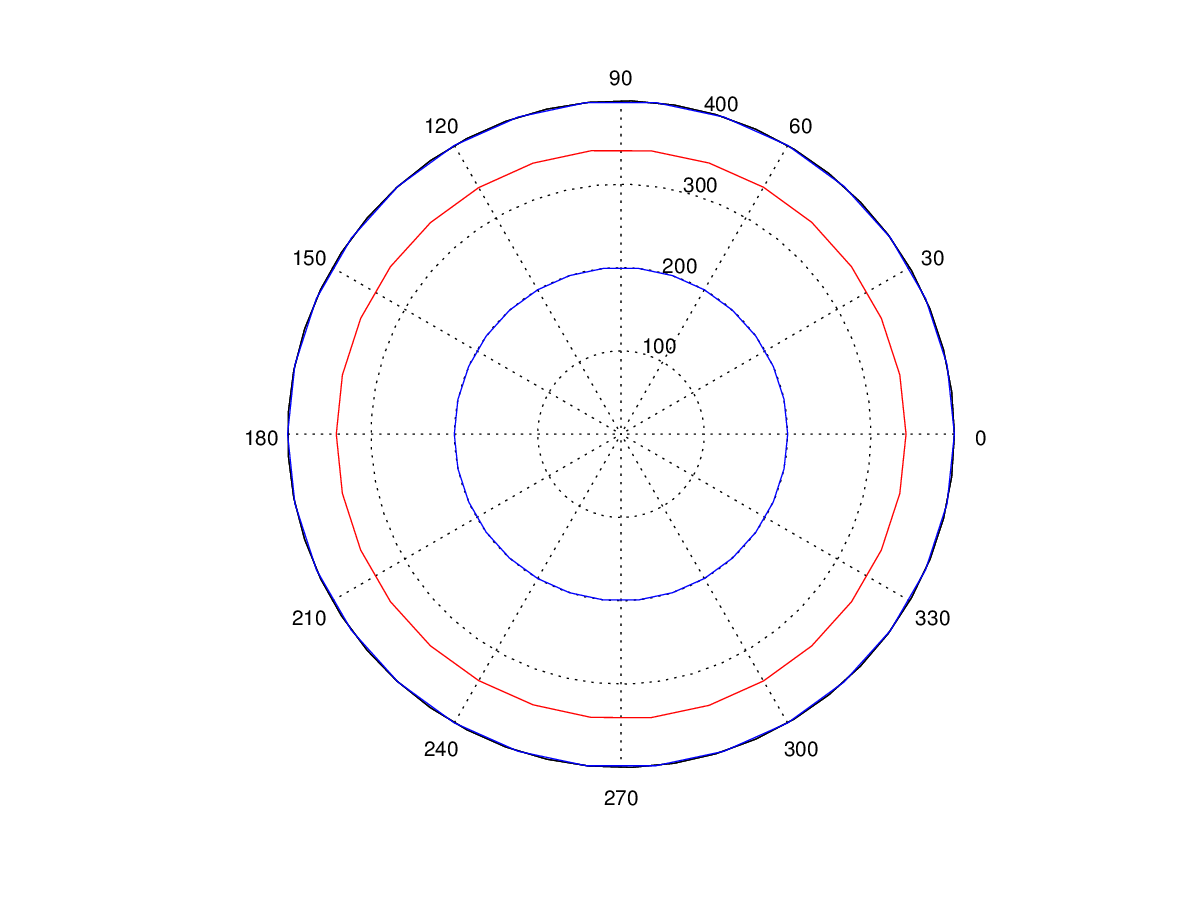
\includegraphics[scale=0.35]{experimentos1a_1b/evolucion_isoterma_cambios_temperatura_varias_discretizaciones/test21_030_radios_030_angulos_inst_001_isomap.png}

	\textbf{Temperaturas externas: } 500\\
	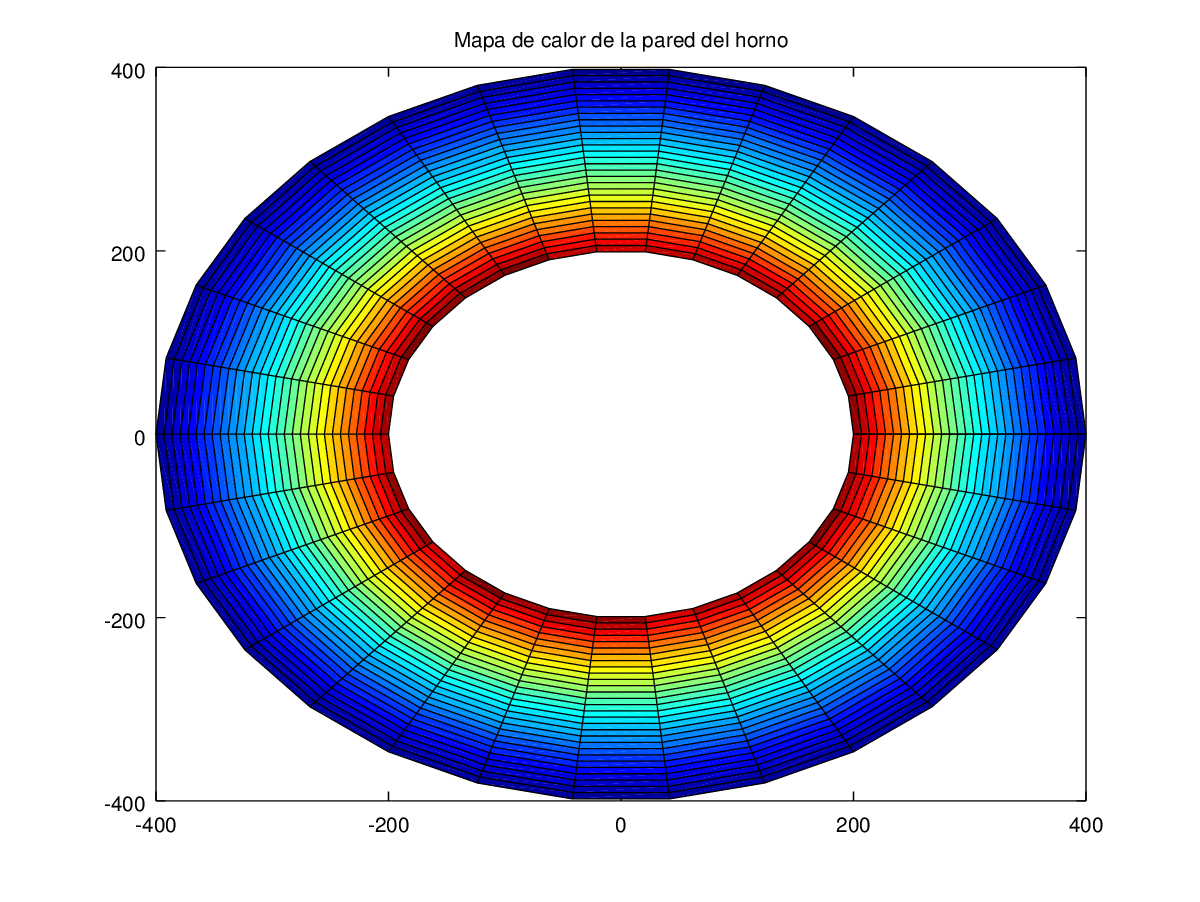
\includegraphics[scale=0.35]{experimentos1a_1b/evolucion_isoterma_cambios_temperatura_varias_discretizaciones/test22_030_radios_030_angulos_inst_001_heatmap.png}
	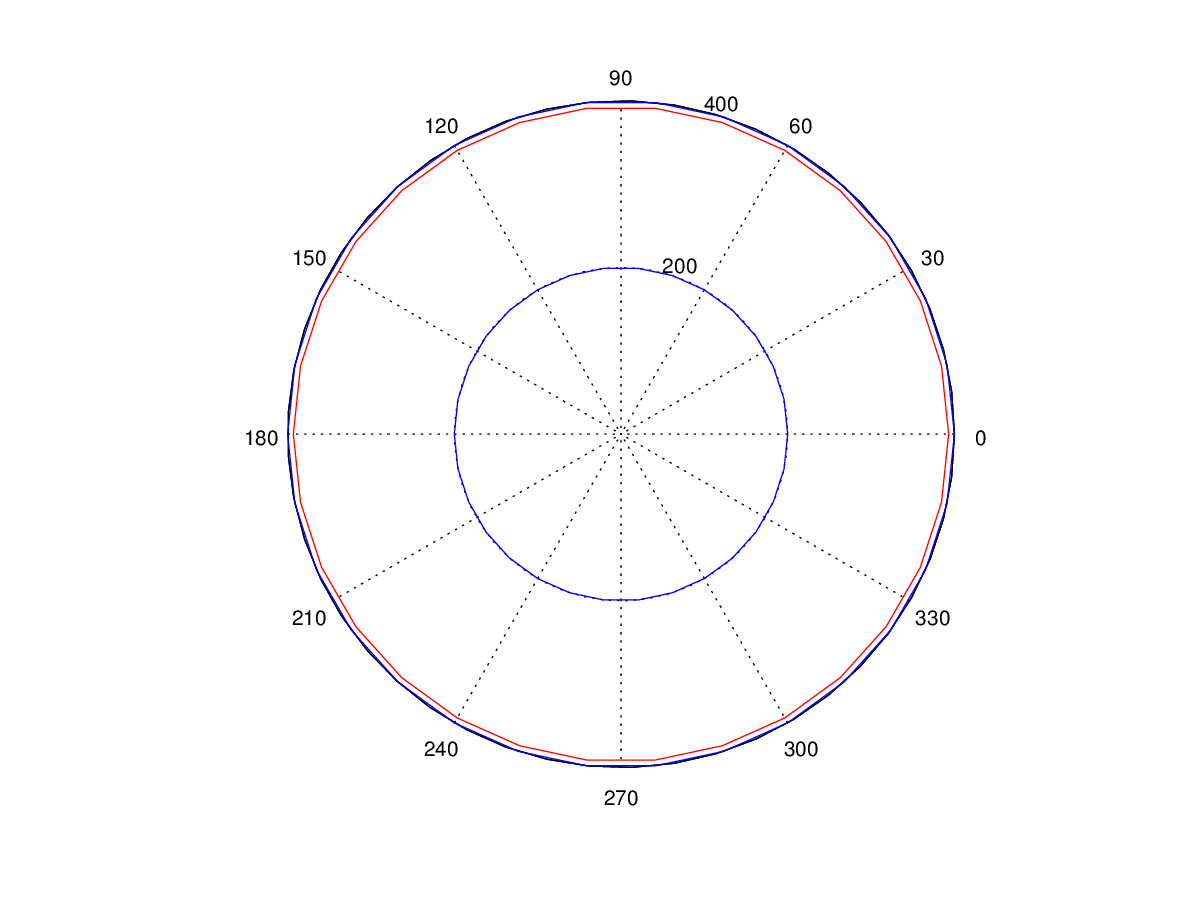
\includegraphics[scale=0.35]{experimentos1a_1b/evolucion_isoterma_cambios_temperatura_varias_discretizaciones/test22_030_radios_030_angulos_inst_001_isomap.png}

	\textbf{Temperaturas externas: } 750\\
	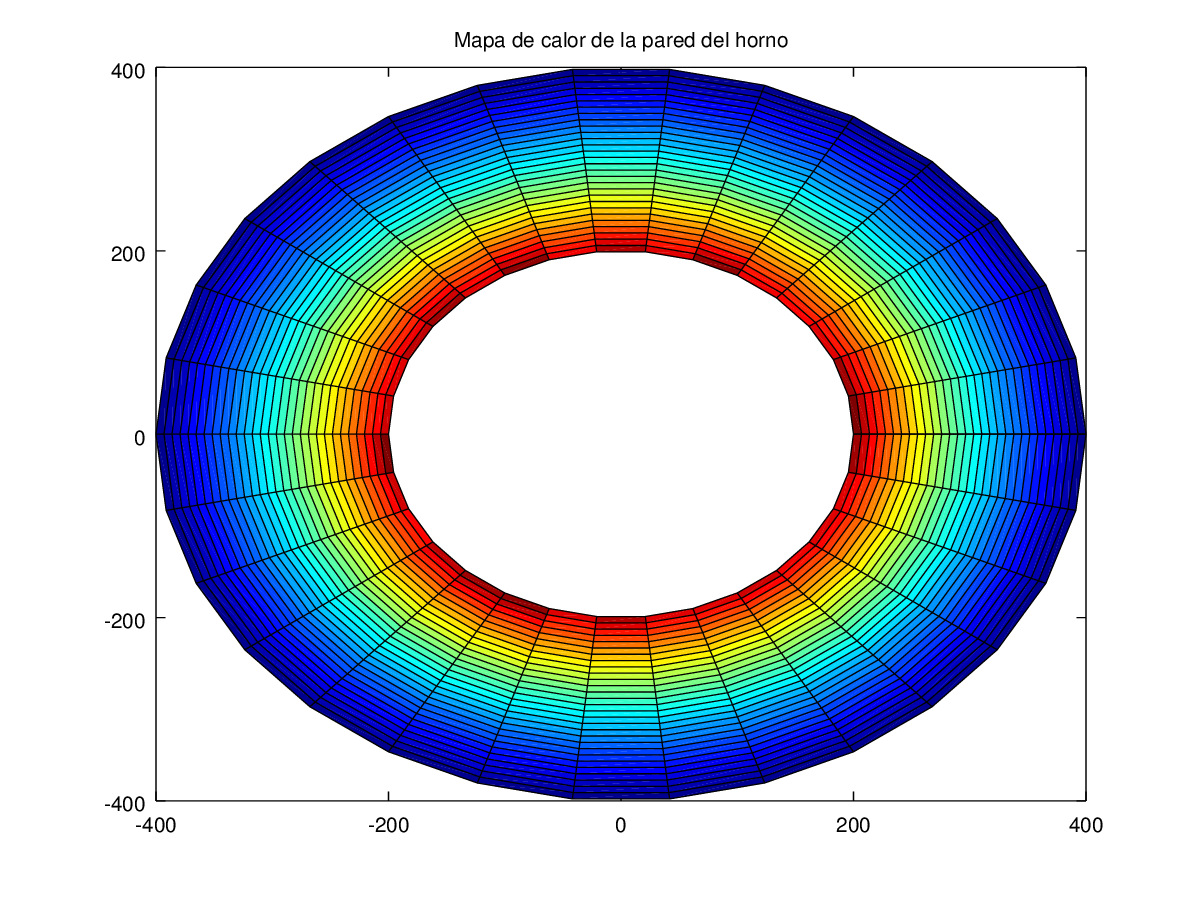
\includegraphics[scale=0.35]{experimentos1a_1b/evolucion_isoterma_cambios_temperatura_varias_discretizaciones/test23_030_radios_030_angulos_inst_001_heatmap.png}
	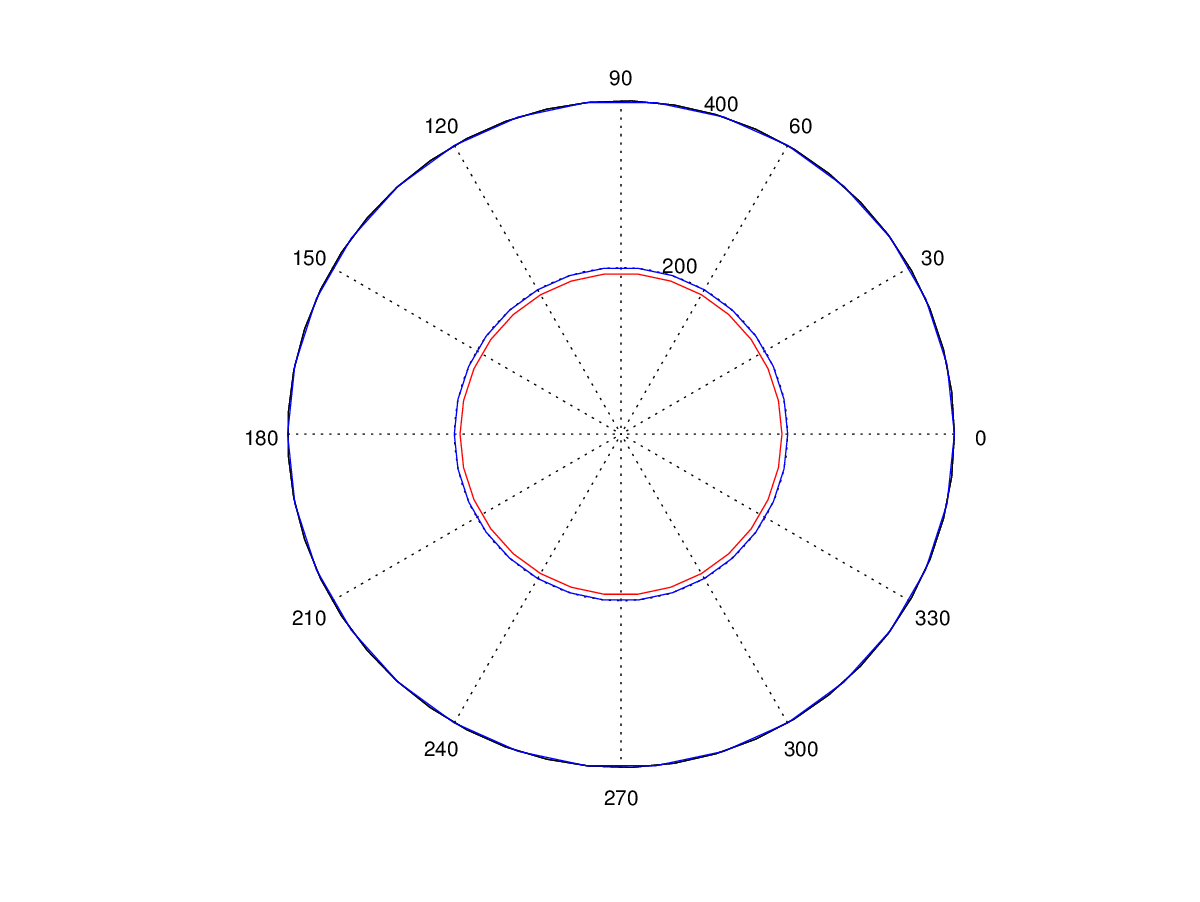
\includegraphics[scale=0.35]{experimentos1a_1b/evolucion_isoterma_cambios_temperatura_varias_discretizaciones/test23_030_radios_030_angulos_inst_001_isomap.png}

\vspace{0.5cm}

La escala de color de los mapas de temperaturas se hace en base al mínimo y máximo de la muestra, es por esto que la variación de temperaturas externas no provee una variación en los colores de los radios del borde. \\
Asimismo, se ve que la posición de la isoterma en los casos $200, 500$ se posiciona según lo esperado dentro de la pared del horno. Mientras que en el caso $750$, al ser $750 > 500$, por convención posicionamos la isoterma en $R_i - \epsilon$.

\vspace{0.5cm}

En la siguiente tabla se puede observar que las métricas de seguridad nos dan una pauta acerca de la posición promedio y maxima de la isoterma dentro de la pared del horno. Si utilizamos $\gamma_0 = 0.75$ como limite de seguridad, podemos establecer conclusiones acerca de la seguridad: en el caso donde hay 200 grados en el exterior es seguro, mientras que 500 grados, no lo es.

\begin{center}
	\begin{tabular}{| c | c | c | c |}
	 	\hline
	 	$T_e$ & $\Delta_{max_{iso500}}$ & $\Delta_{prom_{iso500}}$ & Seguro bajo $\gamma_0 = 0.75$\\
	 	\hline			
		200 & 0.709145 & 0.71037 & Si\\
		\hline
		500 & 0.965517 & 0.965517 & No\\
		\hline  
	\end{tabular}
\end{center}
